
%%%%%%%%%%%%%%%%%%%%%%% file typeinst.tex %%%%%%%%%%%%%%%%%%%%%%%%%
%
% This is the LaTeX source for the instructions to authors using
% the LaTeX document class 'llncs.cls' for contributions to
% the Lecture Notes in Computer Sciences series.
% http://www.springer.com/lncs       Springer Heidelberg 2006/05/04
%
% It may be used as a template for your own input - copy it
% to a new file with a new name and use it as the basis
% for your article.
%
% NB: the document class 'llncs' has its own and detailed documentation, see
% ftp://ftp.springer.de/data/pubftp/pub/tex/latex/llncs/latex2e/llncsdoc.pdf
%
%%%%%%%%%%%%%%%%%%%%%%%%%%%%%%%%%%%%%%%%%%%%%%%%%%%%%%%%%%%%%%%%%%%


\documentclass[runningheads,a4paper]{llncs}

\usepackage{amssymb}
\setcounter{tocdepth}{3}
\usepackage{graphicx}

\usepackage{float}

\def\COM#1{{\color{red}[#1]}}

\usepackage{array}  %pour l'allignement dans les tableaux 


\usepackage[latin1]{inputenc}
\usepackage{times}
\usepackage{helvet}
%package pour les algo
\usepackage{algorithm}
\usepackage{algorithmic}
\usepackage{comment}
%\usepackage{algpseudocode}
%\pagestyle{empty}
%\newcommand{\smallitem}{\vspace*{-2mm}\item}
%\renewcommand{\baselinestretch}{0.95}
%\marginparwidth 0pt 
%\evensidemargin 2.2cm 
%\oddsidemargin 1.8cm 
%\topmargin 0cm 
%\textwidth 12cm 
%\textheight 19cm


%\makeatletter
%\renewcommand{\fnum@figure}{\textbf{\fontsize{10}{10}\selectfont\sffamily\figurename~\thefigure}}
%\renewcommand{\fnum@table}{\textbf{\fontsize{10}{10}\selectfont\sffamily\tablename~\thetable}}
%\makeatother

\begin{comment}
\newcommand{\auteur}[1]{
	\begin{center}
	{#1}
	\end{center}
}

\newcommand{\titre}[1]{
	\begin{center}
	{\large\bfseries \sffamily {#1}}
	\end{center}
}

\newcommand{\affiliation}[1]{
	\noindent
	{\small{#1}}
}
\end{comment}

\usepackage{hyperref}
\usepackage{amsmath}  % Maths
\usepackage{amsfonts} % Maths
\usepackage{amssymb}  % Maths
\usepackage{stmaryrd} % Maths (crochets doubles)

\usepackage{url}     % Mise en forme + liens pour URLs
\usepackage{array}   % Tableaux évolués

\usepackage{prettyref}
\newrefformat{def}{Def.~\ref{#1}}
\newrefformat{fig}{Fig.~\ref{#1}}
\newrefformat{pro}{Property~\ref{#1}}
\newrefformat{pps}{Proposition~\ref{#1}}
\newrefformat{lem}{Lemma~\ref{#1}}
\newrefformat{thm}{Theorem~\ref{#1}}
\newrefformat{sec}{Sect.~\ref{#1}}
\newrefformat{ssec}{Subsect.~\ref{#1}}
\newrefformat{suppl}{Appendix~\ref{#1}}
\newrefformat{eq}{Eq.~\eqref{#1}}
\def\pref{\prettyref}

\usepackage{ntheorem}
\theoremheaderfont{\fontsize{10}{10}\sffamily\bfseries}
%\newtheorem*{example}{Example}{\itshape}{}
\newtheorem{example}{Example}{\itshape}{}
\newtheorem{definition}{Definition}{\itshape}{}


\usepackage{tikz}
\newdimen\pgfex
\newdimen\pgfem
\usetikzlibrary{arrows,shapes}
%\usetikzlibrary{shadows,scopes}
%\usetikzlibrary{positioning}
%\usetikzlibrary{matrix}
%\usetikzlibrary{decorations.text}
%\usetikzlibrary{decorations.pathmorphing}



%\input{macros/macros}

% Macros générales
\def\Pint{\textsc{PINT}}

% Notations générales pour PH
\newcommand{\PH}{\mathcal{PH}}
\newcommand{\PHs}{\Sigma}
\newcommand{\PHl}{L}
\newcommand{\PHp}{\textcolor{red}{\mathcal{P}}}
\newcommand{\PHproc}{\mathcal{P}}
\newcommand{\PHa}{\PHh}
\newcommand{\PHh}{\mathcal{H}}
\newcommand{\PHn}{\mathcal{N}}

\newcommand{\PHhitter}{\mathsf{hitter}}
\newcommand{\PHtarget}{\mathsf{target}}
\newcommand{\PHbounce}{\mathsf{bounce}}
\newcommand{\PHsort}{\Sigma}

\def\f#1{\mathsf{#1}}
\def\focals{\f{focals}}
\def\play{\cdot}
\def\configs#1{\mathbb C_{#1\rightarrow a}}

\newcommand{\PHfrappeA}{\rightarrow}
\newcommand{\PHfrappeB}{\Rsh}
\newcommand{\PHfrappe}[3]{#1\PHfrappeA#2\PHfrappeB#3}
\newcommand{\PHfrappebond}[2]{#1\PHfrappeB#2}
\newcommand{\PHobjectif}[2]{\mbox{$#1\PHfrappeB^*\!#2$}}
\newcommand{\PHconcat}{::}
\newcommand{\PHneutralise}{\rtimes}

\def\PHget#1#2{{#1[#2]}}
\newcommand{\PHchange}[2]{(#1 \Lleftarrow #2)}
\newcommand{\PHarcn}[2]{\mbox{$#1\PHneutralise#2$}}
\newcommand{\PHjoue}{\cdot}

\newcommand{\PHetat}[1]{\mbox{$\langle #1 \rangle$}}

% Notations spécifiques à ce papier
\newcommand{\PHdirectpredec}[1]{\PHs^{-1}(#1)}
\newcommand{\PHpredec}[1]{\f{pred}(#1)}
\newcommand{\PHpredecgene}[1]{\f{reg}({#1})}
\newcommand{\PHpredeccs}[1]{\PHpredec{#1} \setminus \Gamma}

\newcommand{\PHincl}[2]{#1 :: #2}

\def\ctx{\varsigma}
\def\ctxOverride{\Cap}
\def\PHstate#1{\langle #1 \rangle}

\def\DEF{\stackrel{\Delta}=}
\def\EQDEF{\stackrel{\Delta}\Leftrightarrow}

\def\intervalless{<_{[]}}

%\input{macros/macros-ph}

% Notations pour le modèle de Thomas (depuis thèse)
\newcommand{\GRN}{\mathcal{GRN}}
\newcommand{\IG}{\mathcal{G}}
\newcommand{\GRNreg}[1]{\Gamma^{-1}(#1)}
\newcommand{\GRNres}[2]{\mathsf{Res}_{#1}(#2)}
\newcommand{\GRNallres}[1]{\mathsf{Res}_{#1}}
\newcommand{\GRNget}[2]{\PHget{#1}{#2}}
\newcommand{\GRNetat}[1]{\PHetat{#1}}

\def\levels{\mathsf{levels}}
\def\levelsA#1#2{\levels_+(#1\rightarrow #2)}
\def\levelsI#1#2{\levels_-(#1\rightarrow #2)}

\newcommand{\Kinconnu}{\emptyset}
\newcommand{\RRGva}[3]{#1 \stackrel{#2}{\longrightarrow} #3}
\newcommand{\RRGgi}{\mathcal{G}}
\newcommand{\RRGreg}[1]{\RRGgi_{#1}}

\tikzstyle{grn}=[every node/.style={circle,draw=black,outer sep=2pt,minimum
                size=15pt,text=black}, node distance=1.5cm]
\tikzstyle{act}=[->,draw=black,thick,color=black]
\tikzstyle{inh}=[>=|,-|,draw=black,thick, text=black,label]
\tikzstyle{inf}=[->,draw=colorinf,thick,color=colorinf]
\tikzstyle{elabel}=[fill=none,text=black, above=-2pt,%sloped,
minimum size=10pt, outer sep=0, font=\scriptsize, draw=none]
\tikzstyle{sg}=[every node/.style={outer sep=2pt,minimum
                size=15pt,text=black}, node distance=2cm]
                

%Notations pour les patterns dans cytoscape
%%%%%%%%%%%%%%%%%%%%%%%%%%%%%%%%%%%%%%%%%%%%%%%%%%%%%%%%%%%%%%%%%%%%%%%%%%%%%%%%%%%%%%%%%%%
%%%%%%%%%%%%%%%%%%%%%%%%%%%%%%%%%%%%%%%%%%%%%%%%%%%%%%%%%%%%%%%%%%%%%%%%%%%%%%%%%%%%%%%%%%%
%%%%%%%%%%%%%%%%%%Definition des éléments pour un reseau de signalisation%%%%%%%%%%%%%%%%%
\definecolor{pinegreen}{cmyk}{0.92,0,0.59,0.25}
\definecolor{royalblue}{cmyk}{1,0.50,0,0}
\definecolor{lavander}{cmyk}{0,0.48,0,0}
\definecolor{violet}{cmyk}{0.79,0.88,0,0}
\tikzstyle{sn}=[circle, draw, thin,fill=cyan!20, scale=0.8] %seed node
\tikzstyle{ps}=[rectangle, draw, thin,fill=green!20, scale=0.8] %protein de signalisation
\tikzstyle{cplx}=[square, draw, thin, fill=white!20, scale=0.7] %définition d'un complex
\tikzstyle{transl}=[diamond, draw, thin, fill=white!20, scale=0.3]
\tikzstyle{mod}=[triangle, draw, thin, fill=white!20, scale=0.3]
\tikzstyle{qgre}=[rectangle, draw, thin,fill=green!20, size=15pts]
\tikzstyle{tgrn}=[triangle, draw, thin, fill=green!20, scale=0.8]

%Ajout des arc qui ne sont pas définis dans le grn
\tikzstyle{st}=[->, draw, thin, dashed] %définition d'un state transition
\tikzstyle{inhN}=[>=|,-|,draw=colorinh,thick, text=black,label,scale=0.1]
\tikzstyle{actN}=[->,>=triangle 60,draw=coloract,thick,color=coloract,scale=0.1]





%\input{macros/macros-grn}

\usepackage{ifthen}
%\usepackage{tikz}
%\usetikzlibrary{arrows,shapes}

\definecolor{lightgray}{rgb}{0.8,0.8,0.8}
\definecolor{lightgrey}{rgb}{0.8,0.8,0.8}

\tikzstyle{boxed ph}=[]
\tikzstyle{sort}=[fill=lightgray,rounded corners]
\tikzstyle{process}=[circle,draw,minimum size=15pt,fill=white,
font=\footnotesize,inner sep=1pt]
\tikzstyle{black process}=[process, fill=black,text=white, font=\bfseries]
\tikzstyle{gray process}=[process, draw=black, fill=lightgray]
\tikzstyle{current process}=[process, draw=black, fill=lightgray]
\tikzstyle{process box}=[white,draw=black,rounded corners]
\tikzstyle{tick label}=[font=\footnotesize]
\tikzstyle{tick}=[black,-]%,densely dotted]
\tikzstyle{hit}=[->,>=angle 45]
\tikzstyle{selfhit}=[min distance=30pt,curve to]
\tikzstyle{bounce}=[densely dotted,->,>=latex]
\tikzstyle{hl}=[font=\bfseries,very thick]
\tikzstyle{hl2}=[hl]
\tikzstyle{nohl}=[font=\normalfont,thin]

\newcommand{\currentScope}{}
\newcommand{\currentSort}{}
\newcommand{\currentSortLabel}{}
\newcommand{\currentAlign}{}
\newcommand{\currentSize}{}

\newcounter{la}
\newcommand{\TSetSortLabel}[2]{
  \expandafter\repcommand\expandafter{\csname TUserSort@#1\endcsname}{#2}
}
\newcommand{\TSort}[4]{
  \renewcommand{\currentScope}{#1}
  \renewcommand{\currentSort}{#2}
  \renewcommand{\currentSize}{#3}
  \renewcommand{\currentAlign}{#4}
  \ifcsname TUserSort@\currentSort\endcsname
    \renewcommand{\currentSortLabel}{\csname TUserSort@\currentSort\endcsname}
  \else
    \renewcommand{\currentSortLabel}{\currentSort}
  \fi
  \begin{scope}[shift={\currentScope}]
  \ifthenelse{\equal{\currentAlign}{l}}{
    \filldraw[process box] (-0.5,-0.5) rectangle (0.5,\currentSize-0.5);
    \node[sort] at (-0.2,\currentSize-0.4) {\currentSortLabel};
   }{\ifthenelse{\equal{\currentAlign}{r}}{
     \filldraw[process box] (-0.5,-0.5) rectangle (0.5,\currentSize-0.5);
     \node[sort] at (0.2,\currentSize-0.4) {\currentSortLabel};
   }{
    \filldraw[process box] (-0.5,-0.5) rectangle (\currentSize-0.5,0.5);
    \ifthenelse{\equal{\currentAlign}{t}}{
      \node[sort,anchor=east] at (-0.3,0.2) {\currentSortLabel};
    }{
      \node[sort] at (-0.6,-0.2) {\currentSortLabel};
    }
   }}
  \setcounter{la}{\currentSize}
  \addtocounter{la}{-1}
  \foreach \i in {0,...,\value{la}} {
    \TProc{\i}
  }
  \end{scope}
}

\newcommand{\TTickProc}[2]{ % pos, label
  \ifthenelse{\equal{\currentAlign}{l}}{
    \draw[tick] (-0.6,#1) -- (-0.4,#1);
    \node[tick label, anchor=east] at (-0.55,#1) {#2};
   }{\ifthenelse{\equal{\currentAlign}{r}}{
    \draw[tick] (0.6,#1) -- (0.4,#1);
    \node[tick label, anchor=west] at (0.55,#1) {#2};
   }{
    \ifthenelse{\equal{\currentAlign}{t}}{
      \draw[tick] (#1,0.6) -- (#1,0.4);
      \node[tick label, anchor=south] at (#1,0.55) {#2};
    }{
      \draw[tick] (#1,-0.6) -- (#1,-0.4);
      \node[tick label, anchor=north] at (#1,-0.55) {#2};
    }
   }}
}
\newcommand{\TSetTick}[3]{
  \expandafter\repcommand\expandafter{\csname TUserTick@#1_#2\endcsname}{#3}
}

\newcommand{\myProc}[3]{
  \ifcsname TUserTick@\currentSort_#1\endcsname
    \TTickProc{#1}{\csname TUserTick@\currentSort_#1\endcsname}
  \else
    \TTickProc{#1}{#1}
  \fi
  \ifthenelse{\equal{\currentAlign}{l}\or\equal{\currentAlign}{r}}{
    \node[#2] (\currentSort_#1) at (0,#1) {#3};
  }{
    \node[#2] (\currentSort_#1) at (#1,0) {#3};
  }
}
\newcommand{\TSetProcStyle}[2]{
  \expandafter\repcommand\expandafter{\csname TUserProcStyle@#1\endcsname}{#2}
}
\newcommand{\TProc}[1]{
  \ifcsname TUserProcStyle@\currentSort_#1\endcsname
    \myProc{#1}{\csname TUserProcStyle@\currentSort_#1\endcsname}{}
  \else
    \myProc{#1}{process}{}
  \fi
}

\newcommand{\repcommand}[2]{
  \providecommand{#1}{#2}
  \renewcommand{#1}{#2}
}
\newcommand{\THit}[5]{
  \path[hit] (#1) edge[#2] (#3#4);
  \expandafter\repcommand\expandafter{\csname TBounce@#3@#5\endcsname}{#4}
}
\newcommand{\TBounce}[4]{
  (#1\csname TBounce@#1@#3\endcsname) edge[#2] (#3#4)
}

\newcommand{\TState}[1]{
  \foreach \proc in {#1} {
    \node[current process] (\proc) at (\proc.center) {};
  }
}

%%%%%%%%%%%%%%%%%%%%%%%%%%%%%%%%%%%%%%%%%%%%%%%%%%%%%%%%%%%%%%%%%
%% The following definitions are to extend the LaTeX algorithmic 
%% package with SWITCH statements and one-line structures.
%% The extension is by 
%%   Prof. Farn Wang 
%%   Dept. of Electrical Engineering, 
%%   National Taiwan University. 
%% 
\newcommand{\SWITCH}[1]{\STATE \textbf{switch} (#1)}
\newcommand{\ENDSWITCH}{\STATE \textbf{end switch}}
\newcommand{\CASE}[1]{\STATE \textbf{case} #1\textbf{:} \begin{ALC@g}}
\newcommand{\ENDCASE}{\end{ALC@g}}
\newcommand{\CASELINE}[1]{\STATE \textbf{case} #1\textbf{:} }
\newcommand{\DEFAULT}{\STATE \textbf{default:} \begin{ALC@g}}
\newcommand{\ENDDEFAULT}{\end{ALC@g}}
\newcommand{\DEFAULTLINE}[1]{\STATE \textbf{default:} }
%% 
%% End of the LaTeX algorithmic package extension.
%%%%%%%%%%%%%%%%%%%%%%%%%%%%%%%%%%%%%%%%%%%%%%%%%%%%%%%%%%%%%%%%%
\def\layersep{1cm}

\def\modCG#1{\textcolor{red}{#1}}


%pour le texte dans le tableau

\newcolumntype{M}[1]{>{\raggedright}m{#1}}

\usepackage{url}
\urldef{\mailsa}\path|{alfred.hofmann, ursula.barth, ingrid.haas, frank.holzwarth,|
\urldef{\mailsb}\path|anna.kramer, leonie.kunz, christine.reiss, nicole.sator,|
\urldef{\mailsc}\path|louis.fippo-fitime@irccyn.ec-nantes.fr|
\newcommand{\keywords}[1]{\par\addvspace\baselineskip
\noindent\keywordname\enspace\ignorespaces#1}


\begin{document}

\mainmatter  % start of an individual contribution

% first the title is needed
\title{Integrating time-series data in large-scale discrete cell-based models}

% a short form should be given in case it is too long for the running head
\titlerunning{Integrating time-series data in cell-based discrete models}

% the name(s) of the author(s) follow(s) next
%
% NB: Chinese authors should write their first names(s) in front of
% their surnames. This ensures that the names appear correctly in
% the running heads and the author index.
%
\author{Louis Fippo Fitime\inst{1}%
\and Christian Schuster\inst{2} \and Peter Angel\inst{2}
\and Olivier Roux\inst{1}\and Carito Guziolowski\inst{1}}
%
\authorrunning{Louis Fippo Fitime et al.}
% (feature abused for this document to repeat the title also on left hand pages)

% the affiliations are given next; don't give your e-mail address
% unless you accept that it will be published

\institute{LUNAM Universit\'e, \'Ecole Centrale de Nantes, IRCCyN UMR CNRS 6597\\
(Institut de Recherche en Communications et Cybern\'etique de Nantes)\\
1 rue de la No\"e -- B.P. 92101 -- 44321 Nantes Cedex 3, France.\\
\mailsc\\
\url{http://www.irccyn.ec-nantes.fr/en/}
\and
Division of Signal Transduction and Growth Control (A100), DKFZ-ZMBH Alliance, Deutsches Krebsforschungszentrum, Heidelberg, Germany
}

%
% NB: a more complex sample for affiliations and the mapping to the
% corresponding authors can be found in the file "llncs.dem"
% (search for the string "\mainmatter" where a contribution starts).
% "llncs.dem" accompanies the document class "llncs.cls".
%

%\toctitle{Lecture Notes in Computer Science}
%\tocauthor{Authors' Instructions}
\maketitle


\begin{abstract}
In this work we propose an automatic way of generating and verifying 
formal hybrid models of signaling and transcriptional
events, gathered in large-scale regulatory networks.This is done by 
integrating temporal and stochastic aspects of
the expression of some biological components. The hybrid approach lies 
in the fact that measurements take into account both times of 
lengthening phases and discrete switches between them. The model 
proposed is based on a real case study of keratinocytes differentiation, 
in which gene time-series data was generated upon Calcium stimulation.

To achieve this we rely on the Process Hitting (PH) formalism that was 
designed to consider large-scale system analysis.  We first propose an 
automatic way of detecting and translating biological motifs from  the 
Pathway Interaction Database to the PH formalism. Then, we propose a way of estimating 
temporal and stochastic parameters from time-series expression data of 
action on the PH. Simulations emphasize the interest of synchronizing 
concurrent events.
\keywords{time-series data, large-scale network, hybrid models, compositional approach, stochastic simulation}
\end{abstract}



\section{Introduction}

Unraveling and describing the mechanisms involved in the regulation of a cell-based biological system is a fundamental 
issue. These mechanisms can be modeled as biological regulatory networks, whose analysis requires to preliminary build a 
mathematical or computational model. 
By just considering qualitative regulatory effects between components, biological regulatory networks
depict fairly well biological systems, and can be built upon public repositories such as the Pathways 
Interaction Database \cite{schaefer2009pid} and  
hiPathDB \cite{yu2012hipathdb} for human regulatory knowledge.
In this work we built a hybrid model of signaling and transcriptional events, gathered in large-scale regulatory networks, 
for which stochastic simulation parameters were inferred from 
gene expression time-series data.  


High-throughput experimental data has been used since more than one decade ago to infer 
biological regulatory models. 
A variety of methods were proposed to infer dynamic or static models of protein signaling or gene regulations
depending on the nature of the experimental data.
We can cite methods that infer static gene regulatory models from steady-state gene expression datasets of over-expression or knock-down perturbations  
using statistical models generating small-scale (ten species) models \cite{gardner2003inferring} or middle-scale (maximum 100 species) 
models \cite{Pinna2010}.
Additionally, we can cite methods that 
recovered gene regulatory dynamic models from time-series data using kinetic modeling \cite{busch2008gene,porreca2010identification} 
generating small-scale models.
Recently, static boolean models for middle and large-scale (over $100$ species) 
signaling protein networks have been derived from a \emph{prior} network and 
fitted to steady-state multiple perturbation 
phosphoproteomics data \cite{guziolowski2013exhaustively,mitsos2009identifying} using combinatorial optimization through  
logic and integer linear programing to explore the vast search space of candidate boolean models.
When using time-series multi-perturbation phosphoproteomics data, results can be extended to reconstruct middle-scale dynamic signaling models  
via the use of stochastic search approaches \cite{macnamara2012state} that do not guarantee an exhaustive exploration of 
the search space of candidate models.
The approach presented in this work confronts a prior signaling and gene regulatory large-scale network, obtained from publicly curated databases, to 
time-series gene expression data, by using discrete automaton models and stochastic simulations.
Our built model verifies the agreement of expression traces over time given
a signed (activations/inhibitions), directed and cyclic prior graph. 




The advantages and complementariness of our method with respect to the afore cited approaches are that 
it allows us to define a logic that integrates signaling and transcription events (imposing different regulatory rules on these events), 
it also integrates multi-valued states of the system components, and importantly it deals with the complexity of large-scale dynamic models.



Several conceptually different approaches are available for modeling Biological Regulatory Network (BRN) dynamics. The most common approach is ordinary differential equations (ODE) 
that describe deterministic (population average) behavior in a continuous manner. Even for simple models including a simple interaction between two components, 
the analytical solution is impossible. Thus we must refer to simulation as the only practical method. Furthermore, continuous models require quantitative knowledge 
in terms of kinetic coefficients, which are unknown and very difficult to measure. Thereby, various abstraction approaches have been developed to make BRN models 
more convenient for analysis. Synchronous Boolean model was first proposed by Kauffman \cite{kauffman1969metabolic} and an alternative asynchronous model 
was proposed by Thomas \cite{Thomas73}. Following these two papers, many other models have been proposed \cite{snoussi1989qualitative,thieffry1995dynamical,de2003genetic,chaouiya2003qualitative} 
for modeling dynamic of BRN. All of these models are purely qualitative and discrete, thus do not incorporate  quantitative time or other quantities. 
As well, discrete models have been extended to integrate quantitative aspects.  Time aspect have been introduced by \cite{Siebert06,batt2007timed,Ahmad08,van2013timed}. 
It relies on timed automaton implementations. These models, however, do not take into account the stochastic aspects of the influences  of a BRN.




In the context of modeling and analyzing stochastic and concurrent biological systems various formalisms have been introduced such as 
Stochastic Petri Nets which is suitable for the representation of parallel systems \cite{molloy1982performance}. 
They have been successfully applied in many areas; in particular, the specification of Petri Nets
allows an accurate modeling of a wide range of systems including biological systems \cite{heiner2008petri}. The major 
problem of Stochastic Petri Nets is that, generally, they do not lead to compact models. In addition,
they do not provide results to deal with the state space explosion and are thus computationally
expensive when modeling large-scale biological networks. 
The Stochastic pi-calculus formalism was introduced by \cite{priami1995stochastic} and used in 
\cite{maurin2009modeling} for the modeling of biological systems. Stochastic pi-calculus has a rich
expressiveness and is well adapted for the use of compositional approach.
In this work we rely on this formalism through the Process Hitting (PH) framework \cite{PMR10-TCSB}, 
since it is especially useful for studying systems composed of biochemical interactions, and provides
stochastic simulation as well as efficient algorithms, based on the verification of state reachability, to study dynamical properties of the system.
The PH framework uses qualitative and discrete information of the system without requiring enormous parameter estimation tasks
 for its stochastic simulation. 
This framework has been previously used to verify dynamical properties on biological systems without integrating high-throughput experimental data.

In this work we provide a method to build a time-series data integrated PH model and we evaluate 
the prediction power of this model concerning the simultaneously predicted traces of $12$ mRNA expression components of the system upon system stimulation.
The main  results of this work are: (1) automatic generation of PH models integrating gene transcription and signaling events, 
with and without synchronization of concurrent events, from the Pathways Interaction Database, 
(2) parameter estimation from time-series data and parameter integration in the PH model, and
(3) comparison of the PH model predictions and experimental results.
To illustrate our approach, we used a time-series dataset of human keratinocytes cells, which shows
 the fluctuations of mRNA expression across time upon Calcium stimulation.
This dataset was built to study keratinocytes differentiation, a time-dependent
 process in which the sequence of activation of signaling proteins is not yet completely understood.
The method proposed in this paper remains general and can be applied to other case-studies.

%ici je veux présenter la méthodologie et les données que j'ai utilisées 

\section{Data and Methods}

The general workflow for integrating time-series data in a PH model is depicted in \pref{fig:workflow}, in the following sections we 
detail some of the workflow steps.
% and comprises the following steps:
\begin{figure}[H]
 \centering
 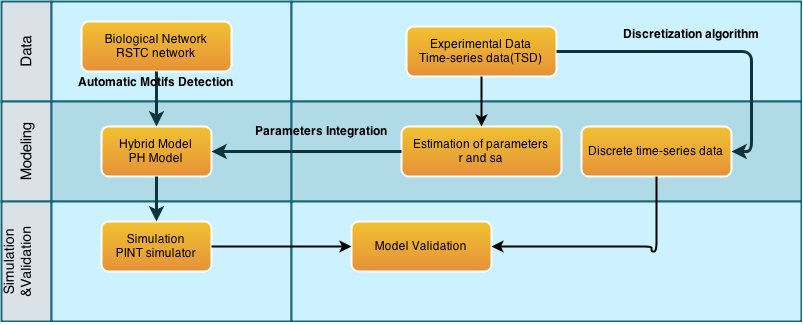
\includegraphics[width=4.1in,height=2in]{images/workflow-2.png}
\caption{{\bf Integrating stochastic and temporal information in a large-scale discrete biological model. The parameters rate (r) and stochasticity absorption factor (sa)  
will be presented later in \ref{sssec:EPTSD}.}} 
 \label{fig:workflow}
\end{figure}


\subsection{Data}

\subsubsection{Interaction graph.}
% \paragraph{The RSTC Network}
\label{ssec:RSTC}


\begin{definition}[Terminal Transient Interaction Graph (TTIG)] \label{def:RSTCDef}
A \emph{TTIG} $N$ is a couple $(V,E)$, where:
\begin{itemize}
\item $V =V_{T} \bigcup V_{I} $ is the finite set of \emph{nodes};
 with 
  $V_{T} = \{v_{1t},v_{2t}, \dots ,v_{n1t} \} $ the set of terminal nodes;
  $V_{I} = \{v_{1i},v_{2i}, \dots ,v_{n2i} \} $ the set of transient nodes.
\item $E = \{e_{1},e_{2}, \dots, e_{m} \}$ is the set of edges. $ E \subseteq (V_{T} \times V_{T}) \bigcup (V_{T} \times V_{I}) 
\bigcup (V_{I} \times V_{T})$
\end{itemize}
\end{definition}

In this definition terminal nodes can be either mRNA expression, proteins,  complexes, cellular states, biological processes or positive conditions. 
On the other side, transient nodes can be either transcriptions or translocations or modifications or compounds. Edges are of different types:
activation (agent), inhibition, output, input and protein-family-member.

\begin{definition}[multi-layer Receptor-Signaling-Transcription-Cell state (RSTC)] 
 A RSTC network is a TTIG were nodes are rallied in layer (Receptor, Signaling, Transcription, Cell state) according to their position in the cell. The position in cell 
 usually induce specific behavior that have to be take into account for modeling. 
\end{definition}



The interactions of the biological system under study were represented in
 a RSTC network, which stands for  multi-layer Receptor-Signaling-Transcription-Cell state network and that was generated from the Pathway Interaction Database (PID).
In order to build this network one needs to select a set of seed nodes related to the biological process studied.
For our case study, the seed nodes were:  (1) \emph{E-cadherin}, which is a protein having Calcium binding domains and which plays an important role in cell adhesion;
(2) the $12$ significantly differentially expressed genes across the $10$ time-points; and (3) the cell states of keratinocytes-differentiation and cell-cycle-arrest. 
The network was extracted automatically from the whole content of the PID database by using a subgraph algorithm to link the seed nodes \cite{guziolowski2012automatic}. 
In \pref{fig:network} we show the RSTC network obtained. 


%\modCG{

\begin{definition}[Pattern] \label{def:pattern}

A pattern can be defined as an atomic set of biological components and their interacting roles. 

\end{definition}


The first column of table \ref{table_patterns} shows  some examples of patterns that can be found in a RSTC Network.

\begin{figure}[!p]
 \centering
 \includegraphics[width=12cm, height=10cm]{images/net_cg_v3.png}
\caption{{\bf  Interaction graph linking E-cadherin with 12 genes of the time-series dataset.} Blue nodes correspond to E-cadherin entities, red or green, to time-series genes, 
and cyan nodes to cellular processes. The graph is composed of $293$ nodes and $375$ edges (interactions).
The set of nodes are composed of terminal nodes (proteins, complexes, mRNA expression, cellular state, biological processes and positive conditions) and of transient
nodes (transcriptions, translocations, modifications and compounds). The set of edges are composed of interactions of type activation, inhibition, output, 
input and protein-family-member.} 
 \label{fig:network}
\end{figure}

%description des données
\subsubsection{Time-series microarray dataset.}
\label{SECTSD}
We use the time-series microarray data from Calcium stimulated human keratinocyte cells 
 measured at $10$ time-points (1h, 2h, 3h, 4h, 5h, 6h, 8h, 12h, 18h, 24h). 
The expression levels were measured in $log_2$; the expression of a gene at an 
specific time point is compared with respect to a control condition (gene expression in a kerationocyte cell without Calcium stimulation).
We selected genes, which mRNA expression $e$ was significantly ($log_2(e) \ge 1$) up-regulated  or 
significantly ($log_2(e) \le -1.0$) down-regulated in at least one time point compared to control.
From this procedure $200$ mRNA expression transcripts were selected. 
We included in our model a subset of $12$ of the $200$ selected (see \pref{fig:tsd})
because these 12 genes had upstream regulatory mechanisms when querying the 
PID database and therefore were connected in the interaction graph to the E-cadherin node.

\begin{figure}[H]
\centering
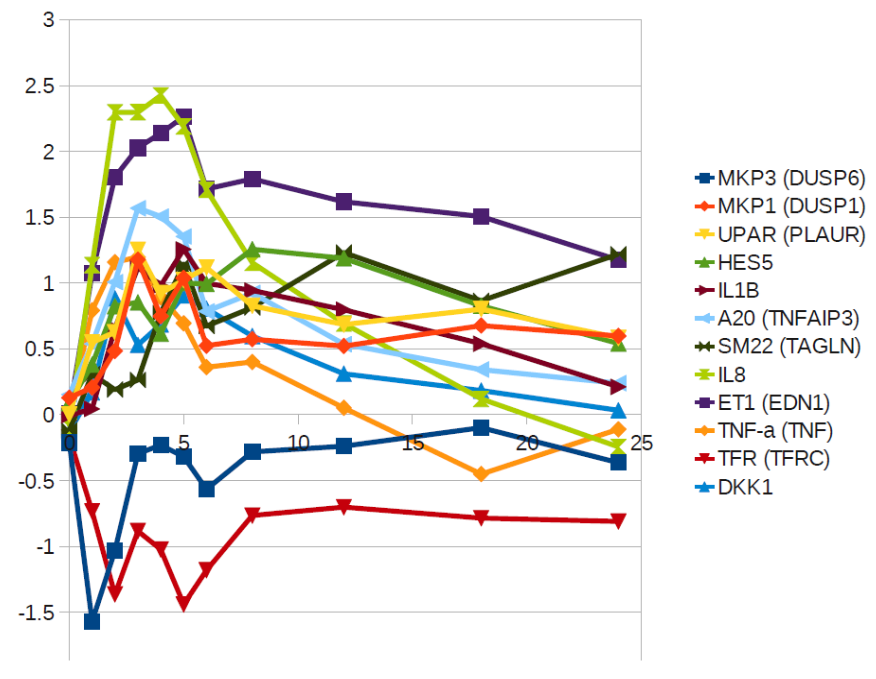
\includegraphics[width=3.5in, height=2.5in]{images/12genes.png}
\caption{\bf Relative expression of selected mRNA upon Calcium stimulation.} The $X$ axis represents time duration of the experiment measured in hours. 
The $Y$ axis represents the $log_{2}$ expression level of genes with respect to control.
\label{fig:tsd}
\end{figure}


\subsection{The Process  Hitting Framework}
\label{ssec:PH}

%We present here the Process Hitting framework \cite{PMR10-TCSB} which will enable us to model 
%biological network.

%\vspace{3mm}
In order to model the dynamics of the system, we use the Process Hitting framework \cite{PMR10-TCSB}.
The Process Hitting (PH) gathers a finite number of concurrent processes grouped into a finite set of sorts.
A sort stands for a component of a biological system while a process, which belongs to a unique sort, stands
for one of its expression levels. At any time exactly one process of each sort is present. A state of the 
PH corresponds to such a set of processes. We denote here a process by $a_i$ where $a$ 
is the sort and $i$ is the process identifier within the sort $a$.
The concurrent interactions between processes are defined by a set of \emph{actions}.
Actions describe the replacement of a process by another of the same sort conditioned by the presence 
of at most one other process in the current state. An action is denoted  $\PHfrappe{a_i}{b_j}{b_k}$, 
which is read as ``$a_i$ \emph{hits} $b_j$ to make it bounce to $b_k$'', where $a_i,b_j,b_k$ are 
processes of sorts $a$ and $b$, called respectively \emph{hitter}, \emph{target} and \emph{bounce} of 
the action.

\begin{definition}[Process Hitting] \label{def:PH}
A \emph{Process Hitting} is a triple $(\PHs,\PHl,\PHa)$, where:
\begin{itemize}
\item $\PHs = \{a,b,\dots\}$ is the finite set of \emph{sorts};
\item $\PHl = \prod_{a\in\PHs} \PHl_a$ is the set of states with $\PHl_a = \{a_0,\dots,a_{l_a}\}$
the finite set of \emph{processes} of sort $a\in\Sigma$ and $l_a$ a positive integer, with $a\neq b\Rightarrow \PHl_a \cap \PHl_b = \emptyset$;
\item $\PHa = \{ \PHfrappe{a_i}{b_j}{b_k} \in \PHl_a \times \PHl_b \times \PHl_b \mid (a,b) \in \PHs^2
  \wedge b_j\neq b_k \wedge a=b\Rightarrow a_i=b_j\}$ is the finite set of \emph{actions}.
\end{itemize}
\end{definition}

\noindent
Given a state $s\in \PHl$, the process of sort $a\in\PHs$ present in $s$ is denoted by $\PHget{s}{a}$.
An action $h=\PHfrappe{a_i}{b_j}{b_k} \in \PHa$ is \emph{playable} in $s \in L$ if and only if $\PHget{s}{a}=a_i$ and $\PHget{s}{b} = b_j$.
In such a case, $(s\play h)$ stands for the state resulting from playing the action $h$ in $s$, with
$\PHget{(s\play h)}{b} = b_k$ and $\forall c \in \PHs, c \neq b, \PHget{(s\play h)}{c} = \PHget{s}{c}$.
In order to model the fact that a molecule in the interaction graph is influenced by various molecules, two 
types of modeling-scenarios can be proposed: cooperation and synchronization.

\subsubsection{Modeling cooperation.}

The cooperation between processes to make another process bounce can be
expressed in PH by building a \emph{cooperative sort}~\cite{PMR10-TCSB}.
\pref{fig:runningPH} shows an example of a cooperative sort $ab$ between sorts $a$ and $b$,
which is composed of 4 processes (one for each sub-state of the presence of processes in $a$ and $b$).
For the sake of clarity, processes of $ab$ are indexed using the sub-state they represent.
Hence, $ab_{01}$ represents the sub-state $\PHstate{a_0,b_1}$, and so on.
Each process of sort $a$ and $b$ hits $ab$, which makes it bounce to the process reflecting the status of the sorts $a$
and $b$ (e.g., $\PHfrappe{a_1}{ab_{00}}{ab_{10}}$ and $\PHfrappe{a_1}{ab_{01}}{ab_{11}}$).
Then, to represent the cooperation between processes $a_1$ and $b_1$,
the process $ab_{11}$ hits $c_1$ to make it bounce to $c_2$ instead of
independent hits from $a_1$ and $b_1$.
The same cooperative sort is used to make $a_0$ and $b_0$ cooperate to hit $c_1$ and make it bounce to $c_0$.
Cooperation sort allows to model the fact that two components cooperate to hit another component.

\subsubsection{Modeling synchronization.}
\label{sssec:synchronization}

The synchronization sort implements another type of cooperation. If we refer to the example of
\pref{fig:runningPH} left, we can similarly construct a \emph{synchronization sort} $ab$ between sorts $a$ and $b$, defined with also 
4 processes. Then, component $c$ is activated ($c_1$ bounces to $c_2$ or $c_0$ bounces to $c_1$) if either  $a$ or $b$ are activated. Therefore, each one of 
these processes $ab_{01}$, $ab_{10}$, $ab_{11}$ can activate $c$.  In order to inhibit $c$, both sorts, $a$ and $b$, need to be 
in the sub-state $0$, i.e. $ab_{00}$. Notice that this rule is a combination of OR logical gates for activation and AND logical gates for inhibition.
Imposing the synchronization sort to model a target component regulated independently by multiple predecessors avoids oscillations in the behavior of the target component over time. 
These oscillations appear because each predecessor can independently activate the target component when it is active,
but when one predecessor is inhibited, it inhibits the target component. This competition between the predecessors
generates oscillations on the target component.  


\begin{example}
\pref{fig:runningPH} represents a PH $(\PHs,\PHl,\PHa)$ with $\PHs = \{a,b,c,ab\}$, and:
\begin{align*}
\PHl_a &= \{a_0,a_1\},\\
\PHl_b &= \{b_0, b_1\},\\
\PHl_{ab} &= \{ab_{00}, ab_{01}, ab_{10}, ab_{11}\},&\\
\PHl_c &= \{c_0, c_1, c_2\}.
\end{align*}
This example models a Biological Regulatory Network (BRN) where the component $c$ has three qualitative levels, components $a$ and $b$ are Boolean and $ab$ is a cooperative sort.
In this BRN, $ab$ inhibits $c$ at level $2$ through the cooperative sort $ab$ (e.g. $\PHfrappe{ab_{00}}{c_2}{c_1}$, $\PHfrappe{ab_{00}}{c_1}{c_0}$) while $a$ and $b$ activate $c$  
through the cooperative sort $ab$ (e.g. $\PHfrappe{ab_{11}}{c_0}{c_1}$ $\PHfrappe{ab_{11}}{c_1}{c_2}$ ). Indeed, the reachability of $c_2$ and $c_0$ 
is conditioned by a cooperation of $a$ and $b$ as explained above.

\begin{figure}[H]
%\centering
\begin{minipage}{0.1\linewidth}
\centering
\scalebox{0.9}{
\begin{tikzpicture}[grn]
\path[use as bounding box] (-0.2,-0.7) rectangle (3.5,0.7);
\node[inner sep=0] (a) at (1,2) {a};
\node[inner sep=0] (b) at (1,0) {b};
\node[inner sep=0] (c) at (3,1) {c};
\path[->]
  (b) edge node[elabel, above=-3pt] {$+$} (c)
  %(c) edge node[elabel, above=-5pt] {$1+$} (a)
  (a) edge node[elabel, above=-3pt] {$+$} (c);
\end{tikzpicture}
}
\end{minipage}
%%%%%%%%%%%%%%%%%%%%%%%%%%%%%%%%%%%%%%%%
\hspace{2cm}
%%%%%%%%%%%%%%%%%%%%%%%%%%%%%%%%%%%%%%%%%
\begin{minipage}{0.7\linewidth}
\centering
\scalebox{0.7}{
\begin{tikzpicture}
\path[use as bounding box] (-2,-5.2) rectangle (7,0.7);

\TSort{(0,0)}{a}{2}{t}
\TSort{(0,-3.8)}{b}{2}{b}
\TSort{(4.5,-3)}{c}{3}{r}

\TSetTick{ab}{0}{00}
\TSetTick{ab}{1}{01}
\TSetTick{ab}{2}{10}
\TSetTick{ab}{3}{11}
\TSort{(-0.5,-2)}{ab}{4}{b}


\THit{a_1}{bend right}{ab_0}{.north}{ab_2}
\THit{a_1}{bend right}{ab_1}{.north}{ab_3}
\THit{a_0}{}{ab_2}{.north west}{ab_0}
\THit{a_0}{}{ab_3}{.north west}{ab_1}

\THit{b_0}{}{ab_1}{.south}{ab_0}
\THit{b_0}{}{ab_3}{.south}{ab_2}
\THit{b_1}{}{ab_0}{.south}{ab_1}
\THit{b_1}{}{ab_2}{.south}{ab_3}

\path[bounce, bend right=25]
\TBounce{ab_2}{}{ab_0}{.north east}
\TBounce{ab_3}{}{ab_1}{.north east}
;
\path[bounce, bend left=80, distance=30]
\TBounce{ab_0}{}{ab_2}{.north}
\TBounce{ab_1}{}{ab_3}{.north}
;
\path[bounce, bend right]
\TBounce{ab_0}{}{ab_1}{.west}
\TBounce{ab_2}{}{ab_3}{.west}
;
\path[bounce, bend left]
\TBounce{ab_3}{}{ab_2}{.east}
\TBounce{ab_1}{}{ab_0}{.east}
;

\THit{ab_3}{thick}{c_1}{.north west}{c_2}
\THit{ab_0}{thick,bend right=130, in=305, distance=140}{c_1}{.south east}{c_0}
\path[bounce, bend left=40]
\TBounce{c_1}{thick}{c_2}{.south west}
\TBounce{c_1}{thick}{c_0}{.north east}
;

\THit{ab_3}{thick}{c_0}{.north west}{c_1}
\THit{ab_0}{thick,bend right=130, in=305, distance=140}{c_2}{.south east}{c_1}
\path[bounce, bend left=40]
\TBounce{c_0}{thick}{c_1}{.south west}
\TBounce{c_2}{thick}{c_1}{.north east}
;
\end{tikzpicture}
}
\end{minipage}

\caption{ \label{fig:modelingBRN}
{\bf (Left)~biological pattern example.}
Nodes represent molecules (components) and edges, interactions.
In this pattern components $a$ and $b$ cooperate to activate $c$.
{\bf (Right)~equivalent PH model} \label{fig:runningPH}
with four sorts: three components ($a$, $b$ and $c$) and a cooperative sort ($ab$).
Actions targeting processes of $c$ are drawn as thick lines.
}
\end{figure}

\end{example}




%la traduction automatique des patterns d'un réseau
\subsection{Model construction (from RSTC to PH)}

\subsubsection{Modeling the RSTC network as a PH model.}

In order to model the RSTC network as a PH model we select known biological regulatory patterns (atomic set of biological components and their interacting roles), represented 
as biochemical reactions in the RSTC network and we propose their PH representation. Table \ref{table_patterns} shows some examples of this transformation. 
The automatic pattern selection and PH model generation algorithms use two procedures. 
The first one takes the graph as parameter argument and automatically browses it node by node and detects all the patterns in the graph. 
For each node (output node of the pattern) we  call a recursive procedure,
that  allows  to detect a minimal set of nodes (input node of the pattern) that has a direct influence over that node. 
This set of nodes plus the output node and the way  input and output are linked form a pattern. 
The type of a pattern is determined by the type of the output node, the type of regulations that come to that node and the type of input nodes of the pattern. 
Consequently, the algorithm of patterns detection returns the pattern 
and its type to another procedure  which  translates the pattern into the PH formalism. This transformation  takes care of different cases (cooperation, synchronization, simple activation, simple inhibition, etc.)
For example a molecule $a$ cooperating with a molecule $b$ to activate a molecule $c$ (\pref{fig:runningPH}, left), is a regulatory pattern because it is a protein-complex biochemical reaction that appears at recurrent times.  
We model this pattern by four sorts (\pref{fig:runningPH}, right) $a$, $b$, $c$ and $ab$. Sorts $a$, $b$ and $c$
stand for components $a$, $b$ and $c$. The cooperative sort $ab$ is introduced in order to characterize constraints on the components $a$ and $b$.
In the RSTC network, we find  $25$ regulatory patterns. We show some examples in Table \ref{table_patterns}.     %TODO

\begin{table}[!t]
\renewcommand{\arraystretch}{1.3}
\caption{Examples of patterns}
\label{table_patterns}
\centering
\begin{tabular}{|c|c|M{4cm}|}
\hline
\bfseries Biological Patterns

&

\bfseries PH Transformations

&

\bfseries Descriptions \tabularnewline 
\hline
\begin{tikzpicture}
\node[scale=0.65] (sa1) at (0,0){\begin{tikzpicture}[auto]
\path[use as bounding box] (-0.7,-0.3) rectangle (2.5,2);

\node[qgre] (a) at (0,1) {a};
\node[mod] (i) at (1,1) {i};
\node[qgre] (b) at (2,1) {b};
\node[es] (d) at (1,1.5) {Simple activation};

\path
 (a) edge[act] (i)
 (i) edge[st]  (b);
\end{tikzpicture}};
\end{tikzpicture}

&


\begin{tikzpicture}
%\exphpatact
\node[scale=0.5] (sa) at (0,0) {\begin{tikzpicture}
\path[use as bounding box] (-0.5,-0.5) rectangle (2.5,2.5);

\TSort{(0,0.5)}{a}{2}{l}
\TSort{(2,0.5)}{b}{2}{l}
%\TSort{(6,1)}{z}{3}{r}

\THit{a_1}{}{b_0}{.west}{b_1}
\THit{a_0}{}{b_1}{.west}{b_0}
%\THit{a_0}{out=250,in=200,selfhit}{a_0}{.west}{a_1}

\path[bounce,bend left]
\TBounce{b_0}{}{b_1}{.south}
\TBounce{b_1}{bend right}{b_0}{.north}
%\TBounce{a_0}{}{a_1}{.south}
;
\end{tikzpicture}};
\end{tikzpicture}

&

This pattern model the activation of the component b by the component a.\tabularnewline
\hline

\begin{tikzpicture}
\node[scale=0.65] (si1) at (0,0){\begin{tikzpicture}[auto]
\path[use as bounding box] (-0.7,-0.3) rectangle (2.5,2);

\node[qgre] (a) at (0,1) {a};
\node[mod] (i) at (1,1) {i};
\node[qgre] (b) at (2,1) {b};
\node[es] (d) at (1,1.5) {Simple inhibition};
\path
 (a) edge[inh] (i)
 (i) edge[st]  (b);
 \end{tikzpicture}};
\end{tikzpicture}

&

\begin{tikzpicture}
%\exphpatact
\node[scale=0.5] (sa) at (0,0) {\begin{tikzpicture}
\path[use as bounding box] (-0.5,-0.5) rectangle (2.5,2.5);

\TSort{(0,0.5)}{a}{2}{l}
\TSort{(2,0.5)}{b}{2}{l}
%\TSort{(6,1)}{z}{3}{r}

\THit{a_1}{}{b_1}{.west}{b_0}
\THit{a_0}{}{b_0}{.west}{b_1}
%\THit{a_0}{out=250,in=200,selfhit}{a_0}{.west}{a_1}

\path[bounce,bend left]
\TBounce{b_1}{bend right}{b_0}{.north}
\TBounce{b_0}{}{b_1}{.south}
%\TBounce{a_0}{}{a_1}{.south}
;
\end{tikzpicture}};
\end{tikzpicture}

&

This pattern model the inhibition of the component b by the component a\tabularnewline
\hline

\begin{tikzpicture}
\node[scale=0.65] (sai1) at (0,0){\begin{tikzpicture}[auto]
\path[use as bounding box] (-0.7,-0.3) rectangle (2.5,3);
\node[qgre] (a) at (0,2) {a};
\node[mod] (i) at (1,1) {i};
\node[qgre] (b) at (0,0) {b};
\node[qgre] (c) at (2,1) {c};
\node[es] (d) at (1,3) {Activation or inhibition};

\path
 (a) edge[act] (i)
 (b) edge[inh] (i)
 (i) edge[st]  (c);
\end{tikzpicture}};
\end{tikzpicture}


&

\begin{tikzpicture}
%\exphpatact
\node[scale=0.5] (sai) at (0,0) {\begin{tikzpicture}
\path[use as bounding box] (-0.5,-0.5) rectangle (2.5,5.5);

\TSort{(0,0)}{a}{2}{l}
\TSort{(0,3)}{b}{2}{l}
\TSort{(2,1)}{c}{2}{r}

\THit{a_1}{}{c_0}{.west}{c_1}
\THit{a_0}{}{c_1}{.west}{c_0}
\THit{b_1}{}{c_1}{.west}{c_0}
\THit{b_0}{}{c_0}{.west}{c_1}

%\THit{a_0}{out=250,in=200,selfhit}{a_0}{.west}{a_1}

\path[bounce,bend left]
\TBounce{c_1}{bend right}{c_0}{.north}
\TBounce{c_0}{}{c_1}{.south}
%\TBounce{a_0}{}{a_1}{.south}
;
\end{tikzpicture}};
\end{tikzpicture} 

&

This pattern model either the activation of the component c by the component a or the inhibition of the 
component c by the component b \tabularnewline
\hline
\end{tabular}
\end{table}


%%%%%%%%%%%%%%%%%%%%%%%%%%%%%%%%%%%%%%%%%%%%%%%%%%%%%%%%%%%%%%%%%%%%%%%%%%

\subsubsection{Estimating the parameters for the PH-simulation from time-series gene expression data.}
\label{sssec:EPTSD}
%peut etre penser à faire un schéma

Since the simulation of the execution of the PH actions is done stochastically, we need to relate each action with temporal 
and stochastic parameters introduced into the PH framework to achieve dynamic refinement \cite{PMR10-TCSB}. 
To fire an action in the PH framework we need to provide two parameters: (1) the rate $r=t^{-1}$, where $t$ is the mean time for firing an action,
and (2) the stochasticity absorption factor $sa$, which is introduced to control the variance of firing time of an action.


\begin{figure}[H]
\centering

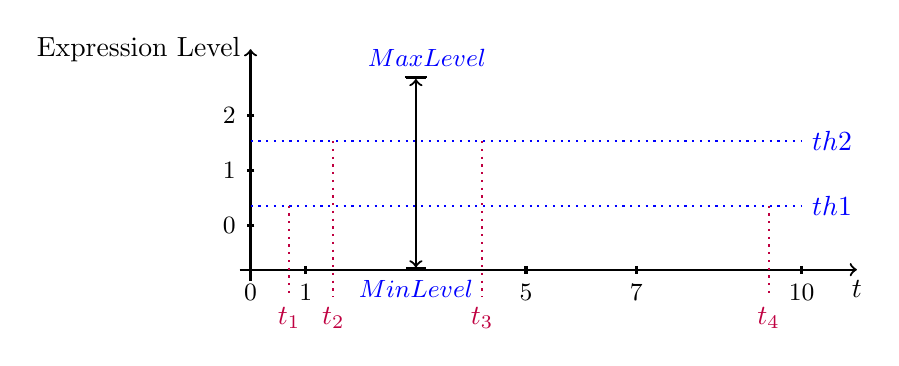
\begin{tikzpicture}[scale = 0.7]
       
    
	      \draw[thick, ->] (-.2,0)--(11,0) node[below]{$t$};
	      \foreach \t in {0,1,5,7,10}
	      \draw[very thick] (\t,2pt)--(\t,-2pt) node[below,black]{\small\t};

	      \draw[thick, ->] (0,-.2)--(0,4) node[left]{Expression Level};
	      \foreach \y in {0,1,2}
               \draw[very thick] (2pt, \y+0.8 )--(-2pt, \y+0.8 ) node[left,black]{\small\y};
           
	      \draw[thick] plot[mark=ball,mark size=1pt] file {illustration.txt};
    
	      %\pause
	      \draw[thick] (2.8,3.5) -- (3.2,3.5) node[above,blue]{\small $MaxLevel$};
	      %\draw[thick,|<->|] (-.2,-.2) -- (.2,-.2) node[below,blue]{};
	      %\pause
	      \draw[thick,|<->|] (3,0)node[below,blue]{\small $MinLevel$} -- (3,3.5);
	      %\pause
	      \draw[thick,dotted,blue] (0,1.16) -- (10,1.16) node[right]{$th1$}; 
	      \draw[thick,dotted,blue] (0,2.33) -- (10,2.33) node[right]{$th2$}; 
	      %\pause
	      \draw[thick,dotted,purple] (0.7,1.16) -- (0.7,-.5) node[below]{$t_{1}$};
	      %\pause
	      \draw[thick,dotted,purple] (1.5,2.33) -- (1.5,-.5) node[below]{$t_{2}$};
	      %\pause
	      \draw[thick,dotted,purple] (4.2,2.33) -- (4.2,-.5) node[below]{$t_{3}$};
	      %\pause
	      \draw[thick,dotted,purple] (9.4,1.16) -- (9.4,-.5) node[below]{$t_{4}$};

           \end{tikzpicture}
	    

\caption{{\bf Estimating temporal parameters from time series data:} The mean firing time of an action that makes a
component (mRNA expression) change of sub-state is estimated as $r_{i}=\frac{1}{t_{i}-t_{i-1}}$. $MaxLevel$ represents the maximum expression of a mRNA expression, while 
 $MinLevel$, its minimum expression.
The thresholds $th1$ and $th2$ define the PH discrete sub-states (e.g. 0,1,2) of a component according to its gene expression data.
\label{fig:estimationParameter}}
\end{figure}


For the model components which have a measurement in the time-series data we estimate the $r$ and $sa$ parameters and they are introduced in the PH model. 
The other components are 
assigned default parameters. In order to estimate $r_{i}$ and $sa_{i}$ for each action $h_{i} \in \PHa$, we need to know the different times $t_{i}$  when the action could be fired as illustrated 
in \pref{fig:estimationParameter}. Each  $t_{i}$ represents the time at which we assume that a component moves from one process to another. Therefore the action that leads this 
change must be played at the rate $r_{i}=\frac{1}{t_{i}-t_{i-1}}$. The integer $sa$ represents the window of firing the action at rate $r$ : the larger the $sa$ is, the smaller the variance around $r$ is. 
Studies \cite{AMSW2012,Batt15092010,RAT2006} have proposed more elaborated methods for parameters estimation from gene expression data. These methods are well adapted in the case of biochemical reactions where 
the concept of threshold is implicit. In the proposed case we assume an explicit threshold. Thus a basic estimation algorithm can be used for temporal and stochastic parameter estimation.

%discretisation des données
\subsubsection{Discretization of time-series data.}

Because the outputs of a PH simulation are discrete traces of PH components, we discretized continuous experimental data to facilitate 
the comparison with simulation outputs.
When looking at the time-series data (see \pref{fig:tsd}) one can distinguish a high level of
activity in early hours [$0h$-$5h$] and a low level in late hours [$5h$-$10h$]. This trend was confirmed by the SMA (Simple moving average) function of the R package TTR which allows us
to smooth time-series data. We used the SMA function with parameter $n=2$ and we observed that more than $50\%$ of the time-series data presented these two levels of activities.
We implemented a discretization method to capture these
two activation times. For each time-series, we introduced two thresholds \emph{th1} and \emph{th2} (see \pref{fig:estimationParameter}) were introduced: 
$\emph{th1}=\frac{1}{3}(MaxLevel-MinLevel)$ and $\emph{th2}=\frac{2}{3}(MaxLevel-MinLevel)$. 
In this way, the expression level in the range $[0-th1]$ is at level $0$, the one in the range $[th1-th2]$ is at level $1$, and the one in the last range is at
level $2$. 


\subsection{Simulation}

We set the same initial conditions to PH components belonging to the same network layer, chosen from the RSTC structure.
These initial conditions are detailed below and summarized in \pref{fig:initialCondition}.
\begin{itemize}
 \item \textbf{Receptor layer: E-cadherin.} We choose the  pulse signal for the input node E-cadherin to be active for a duration of $5$ time units in average. This 
 choice was made in orders to take into account the average time of the Calcium stimuli effect.
 \item \textbf{Signaling layer: signaling proteins.} The components in this layer are activated and inhibited with the same rate and the same stochasticity absorption factor. 
The actions between a controller component $A$ and a controlled component $B$ are constrained so that 
$B$ is first activated by $A$ and then inhibited.  That is, 
the time interval in which an inhibition action from $A$ to $B$ fires is greater than 
the time interval in which an activation action from $A$ to $B$ fires.
Additionally, these two time intervals must not overlap.
These constraints can be seen as 
reachability constraints from the entry  node (E-cadherin) to the output nodes (mRNA expression). The values of these parameters are selected by considering the delay of signal transduction from the entry
 node to the output nodes.
 \item \textbf{Transcription layer: transcription factors.} In this layer, the activation/inhibition over a transcription factor (TF) comes from signaling proteins; however, 
for all TFs we introduced an auto-inhibition action that represents their degradation over time. 
 \item \textbf{mRNA expression.} The mRNA expression are activated or inhibited according to the estimated values from time-series data.
\end{itemize}


\begin{figure}[H]
 
 \centering
 \scalebox{0.65}{
% \begin{comment}
  \begin{tikzpicture}[shorten >=1pt,->,draw=black!50, node distance=\layersep]
  
    \tikzstyle{every pin edge}=[<-,shorten <=1pt];
    \tikzstyle{neuron}=[circle,fill=black!25,minimum size=17pt,inner sep=0pt]
    \tikzstyle{input neuron}=[neuron, fill=green!50];
    \tikzstyle{output neuron}=[neuron, fill=red!50];
    \tikzstyle{hidden neuron}=[neuron, fill=blue!50];
    \tikzstyle{transfact neuron}=[neuron, fill=blue!20];
    \tikzstyle{annot} = [text width=4em, text centered];

    % Draw the input layer nodes
    \foreach \name / \x in {1,...,5}
    % This is the same as writing \foreach \name / \y in {1/1,2/2,3/3,4/4}
       % \node[input neuron, pin=left:Output \#\y] (I-\name) at (0,-\y) {};
         \node[input neuron] (I-\name) at (\x-7,-4) {};

     % Draw the transcription factor layer node
    \foreach \name / \x in {1,...,5}
    % This is the same as writing \foreach \name / \y in {1/1,2/2,3/3,4/4}
       % \node[input neuron, pin=left:Output \#\y] (I-\name) at (0,-\y) {};
         \node[transfact neuron] (TF-\name) at (\x-7,-2) {};
     
     
     % Draw the hidden layer nodes
    \foreach \name / \x in {1,...,5}
        \path[yshift=0.5cm]
           % node[hidden neuron] (H-\name) at (\layersep,-\y cm) {};
             node[hidden neuron] (H-\name) at (\x-7 , \layersep) {};
             
    
    % Draw the hidden layer nodes
    \foreach \name / \x in {1,...,5}
        \path[yshift=0.5cm]
           % node[hidden neuron] (H-\name) at (\layersep,-\y cm) {};
             node[hidden neuron] (H1-\name) at (\x-7 ,1) {};
             
     % Draw the hidden layer nodes 1
    \foreach \name / \x in {1,...,5}
        \path[yshift=0.5cm]
           % node[hidden neuron] (H-\name) at (\layersep,-\y cm) {};
             node[hidden neuron] (H2-\name) at (\x-7 ,0) {};
             
     % Draw the hidden layer nodes 2
    \foreach \name / \x in {1,...,5}
        \path[yshift=0.5cm]
           % node[hidden neuron] (H-\name) at (\layersep,-\y cm) {};
             node[hidden neuron] (H3-\name) at (\x-7 ,-1) {};
             
    % Draw the output layer node
     \node[output neuron,pin={[pin edge={<-}]right:Stimuli}] (O) at (2.5-8,4.5) {};
     
     
   %connect nodes   

    % Connect every node in the input layer with every node in the
    % hidden layer.
    \foreach \source in {1,3,5}
        \foreach \dest in {1,...,5}
            \path (H-\dest) edge (H3-\source);

    % Connect every node in the hidden layer with the output layer
    \foreach \source in {1,...,5}
        \path (O) edge (H-\source) ;
        
   %connect sp to tf
   \foreach \source in {1,...,5}
    \path (H3-\source) edge (TF-\source);
        
    %connect TF with Genes
    
    \foreach \source in {1,...,5}
     \path (TF-\source) edge (I-\source);

   %add some feedbacks 
    
    \path (I-5) edge[inh, bend right] (H-5);
    \path (I-1) edge[inh, bend left] (H3-1);
    \path (I-3) edge[inh] (H3-2);
     
      %titre du graphe
    \node[annot] (graphTitle) at (2.5-7,7) {\textcolor{blue}{\large \textbf Graph Structure}};

    % Annotate the layers
    \node[annot] (layerTitle) at (-9,7) {\textcolor{blue}{\large \textbf Layer}};
    \node[annot, node distance=1cm] (couchesp) at (-9,1) {\large \textbf{Signaling Proteins}};
    \node[annot] (coucheFT) at (-9,-2) {\large \textbf{TF} };
    \node[annot] (coucheGene) at (-9,-4) {\large \textbf{Genes} Output };
    \node[annot] (noeudEntre) at (-9,5) {\large \textbf{Ecad} Input };
    
    %noeud pour ajouter le R S T C 
    \node[annot] (R) at (-11,5) {\textcolor{black}{\textbf \LARGE R}};
    \node[annot] (S) at (-11,1) {\textcolor{black}{\textbf \LARGE S}};
    \node[annot] (T) at (-11,-2) {\textcolor{black}{\textbf \LARGE T}};
    \node[annot] (C) at (-11,-4) {\textcolor{black}{\textbf \LARGE C}};
    \node[annot] (test) at (5,-4) {\textcolor{black}{\textbf -}};
    
    %noeud pour les règles de modélisation
    \node[annot] (icTitle) at (0,7) {\textcolor{blue}{\textbf \large Initial Conditions}};
    \node[annot] (RMi) at (0,4.5) {\textcolor{black}{\textbf \LARGE 1}};
    \node[annot] (SMi) at (0,1) {\textcolor{black}{\textbf \LARGE 0}};
    \node[annot] (TMi) at (0,-2) {\textcolor{black}{\textbf \LARGE 0}};
    \node[annot] (CMi) at (0,-4) {\textcolor{black}{\textbf \LARGE 0}};
    %\node[annot] (P) at (5,-4) {\textcolor{black}{\huge \textbf{}}};
    
    %noeuds pour les hypothèses de modélisation 
    \node[annot] (parameterTitle) at (3,7) {\textcolor{blue}{\textbf \large Parameters}};   %text width=3cm
    \node[annot] (RH) at (3,5) {\textcolor{black}{\textbf \LARGE -}};
    \node[annot] (SH) at (3,1) {\textcolor{black}{\small \textbf \LARGE r=$10$ - sa=$50$}};
    \node[annot] (TH) at (3,-2) {\textcolor{black}{\small \textbf \LARGE r=$10$ - sa=$50$}};
    \node[annot] (CH) at (3,-4) {\textcolor{black}{\small \textbf \large learned from TSD}};
    %\node[annot] (test) at (5,-4) {\textcolor{black}{\huge \textbf{}}};
    
    %noeuds de repères pour les sous-graphs
    
    \node[annot] (R1) at (-4.7,\layersep) {};
    \node[annot] (R2) at (-4.7,1) {};
    \node[annot] (R3) at (-6.8,-1) {};
    \node[annot] (R4) at (-6.5,-4) {};
    \node[annot] (R5) at (-6.5,\layersep) {};
    
   

\end{tikzpicture}
}

 \caption{\bf RSTC network structure and initial conditions assigned to each node in the layer}
 \label{fig:initialCondition}

 
 \end{figure}


\begin{comment}
\begin{figure}
 
\begin{tikzpicture}[auto]

\node[qgre] (a1) at (-3,-3) {a};
\node[qgre] (a2) at (-1,-3) {b};
\node[qgre] (a3) at (1,-3) {c};
\node[qgre] (a4) at (3,-3) {d};
%\node[qgre] (a5) at (5,-3) {e};

\node[mod] (i1) at (-3,-2) {};
\node[mod] (i2) at (-1,-2) {};
\node[mod] (i3) at (1,-2) {};
\node[mod] (i4) at (3,-2) {};
%\node[mod] (i5) at (5,-2) {};

\node[ps] (ps1) at (-3,-1) {PS1};
\node[ps] (ps2) at (-1,-1) {PS2};
\node[ps] (ps3) at (1,-1) {PS3};
\node[ps] (ps4) at (3,-1) {PS4};
%\node[ps] (ps5) at (5,-1) {PS5};

\node[mod] (i6) at (-3,0) {};
%\node[mod] (i7) at (-1,0) {};
\node[mod] (i8) at (1,0) {};
\node[mod] (i9) at (3,0) {};
%\node[mod] (i10) at (5,0) {};

\node[ps] (ps6) at (-3,1) {PS6};
%\node[ps] (ps7) at (-1,1) {PS7};
\node[ps] (ps8) at (1,1) {PS8};
\node[ps] (ps9) at (3,1) {PS9};
%\node[ps] (ps10) at (5,1) {PS10};

%les complex
\node[ecad] (d) at (0,3) {Ecad};
\node[cplx] (c1) at (2,-1) {cplx1};
\node[cplx] (c2) at (0,1) {cplx2};
\node[cplx] (c3) at (-2,-1) {cplx3};
\node[cplx] (c4) at (-2,1) {cplx4};
\node[cplx] (c5) at (0,0) {cplx5};
\node[cplx] (c6) at (2,1) {cplx6};

%les seed node
\node[sn] (sn1) at (-2,-3) {SN1};
\node[sn] (sn2) at (2,-3) {SN2};


%les edges 

\path
 (i1) edge[st] (a1)
 (i2) edge[st] (a2)
 (i3) edge[st]  (a3)
 (i4) edge[st]  (a4)
 %(i5) edge[st]  (a5)
 
 (ps1) edge[act] (i1)
 (ps2) edge[act] (i2)
 (ps3) edge[act] (i2)
 (ps3) edge[act] (i3)
 (ps4) edge[act] (i4)
 %(ps5) edge[act] (i5)
 
 (i6) edge[st] (ps1)
 (i6) edge[st] (ps2)
 (i8) edge[st] (ps3)
 (i9) edge[st] (ps4)
 (i9) edge[st] (ps4)
 %(i9) edge[st] (ps5)
 %(i10) edge[st] (ps5)
 
 (ps6) edge[act] (i6)
 (ps8) edge[act] (i8)
 (ps9) edge[act] (i9)
 %(ps10) edge[act] (i10)
 
 (d) edge[act] (ps6)
 (d) edge[act] (ps8)
 (d) edge[act] (ps9)
 %(d) edge[act] (ps10)
 
 (c4) edge[act] (c5)
 (c2) edge[act] (c5)
 (d) edge[act] (c2)
 (c5) edge[inh] (ps2)
 (c6) edge[act] (i8)
 (c6) edge[act] (i9)
 (i8) edge[st] (c1)
 (i9) edge[st] (c1)
 (c1) edge[act] (i4)
 
 (ps3) edge[inh] (sn2)
 (i4) edge[st] (sn2)
 
 (ps1) edge[inh] (sn1)
 (c3) edge[act] (sn1)
 (c4) edge[act] (c3)
 
 (a1) edge[inh, bend left] (ps6);
 
\end{tikzpicture}

\caption{\bf RSTC network structure and initial conditions assigned to each node in the layer}
 \label{fig:initialCondition}


\end{figure}

\end{comment}
 
 %model validation
 \subsection{Automatic analysis of simulation traces}
 
 Due to the stochastic and concurrent aspects of the system, each execution of the model can generate a different dynamic trace.
 Therefore, to validate the proposed model, we analyzed the traces generated by each component for a set of simulations of the model.
 The idea was to calculate the percentage of traces that reproduced the expected dynamic of the system. 
To achieve this goal, we take each trace generated
 at each simulation for a given component and passed it to an automaton ($\mathcal{A}_{i}$) that recognize the 
experimental trace of that component. Thus we can count the 
 number of accepted traces ($Trace_{accp}$);
the percentage of accepted traces is $\frac{Trace_{accp}}{Trace_{N}}$ if we assume that $Trace_{N}$ is the total 
 number of simulations. 
 Following this we introduce the concept of tolerance in accepting traces. It means that an automaton can accept a trace with a difference 
 of one or more levels at each state. In our case study we used a tolerance $T_{1}$ that allows accepting a difference of one between the 
simulated trace and the expected trace at each state.
 

%fin de methods.

\section{Results}
\subsection{Automatic generation of PH model from the PID network}
%give statistics
PH models are written using the PINT\footnote{\url{http://process.hitting.free.fr}} format.  
PINT implements stochastic simulations and static analyses for computing dynamical properties on very large-scale PH models.
For the PINT code generation two procedures were used.
The first procedure detects motifs (controller and controlled components) in graphs from the Pathway Interaction Database; the second, 
generates the PINT code by choosing an adequate concurrency rule, based on synchronization sorts, to represent the motif dynamic in PH.
With this method it is possible to convert the whole content of the PID database into a PH model, as well as individual pre-selected pathways, 
as is the case for the system under study.  It is implemented in Java and available upon request.

\subsection{Simulation of Calcium stimulated biological system}
We simulated the model with and without the inclusion of the synchronization sort. In the following, we present the results of 
the simulation.

\subsubsection{Without the introduction of the synchronization sort.}
One can notice in \pref{fig:rwos} the occurrence of oscillations. Whereas it is not the expected behavior from the biological system,
 it is coherent with the choice of the modeling and the way the simulator works as explained in Section \ref{sssec:synchronization}.
In this simulation, cooperation sorts were used to model multiple controllers of a common controlled (target) component.
It is important to notice that the intensity of the oscillation is linked with 
the size of the concurrence, i.e. the number of controllers a controlled component has.
Despite the presence of the oscillations, the model reproduces expected dynamical behaviors  namely
the dynamics of components, the signal transduction and takes into account the stochastic and time aspect of the model.

\begin{figure}[H]
\centering
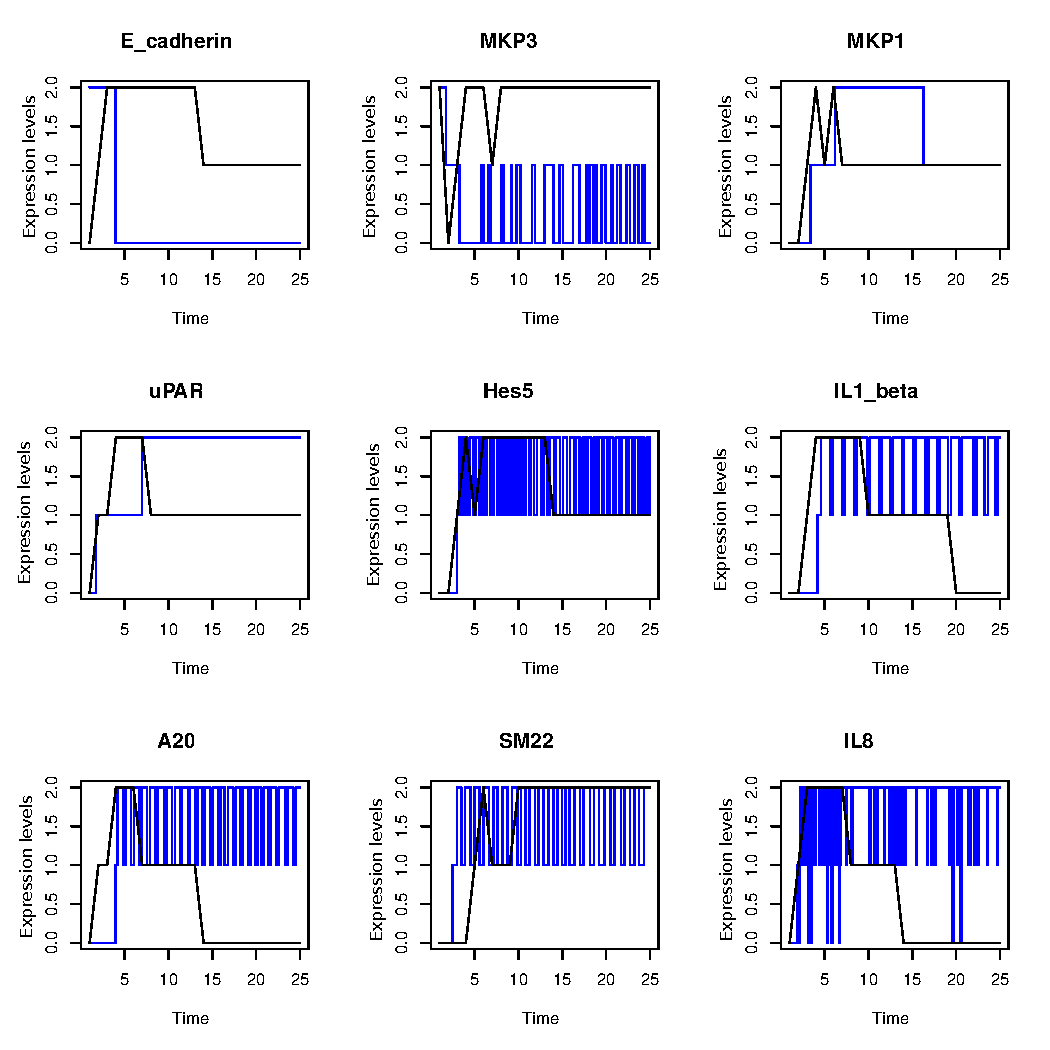
\includegraphics[width=5in,height=4in]{images/resultWOS.pdf}
\caption{{\bf Results of system simulations without introducing the synchronization sort for 9 genes.} The 
traces representing the discretized time-series data are shown as black lines.  The traces representing the simulated traces are shown as blue lines.}
\label{fig:rwos}
\end{figure}

\subsubsection{With the introduction of the synchronization sort.}
In \pref{fig:rws} we can see that the introduction of the synchronization sort significantly reduces the 
impact of concurrency. The result shows  a 
clear elimination of the previously observed oscillations (\pref{fig:rwos}). 
Comparing the simulated results with the ones observed experimentally, we found four different cases.
We found $5$ simulation traces (IL8, uPAR, IL1\_beta, ET1, A20) that matched the sequence of all the component expression levels perfectly.  In this case, delays exist among simulation and experiment but 
these delays are not comparable since experimental time-points are measured in hours and simulation-units for the simulated PH model.
We found $6$ simulation traces (MKP1, MKP3, Hes5, SM22, TfR, DKK1) that matched the sequence of experimental discrete expression levels missing one expression-level.
We found $1$ components (TNF-alpha) in which at least 2 expression levels are missed.

\begin{figure}[H]
\centering
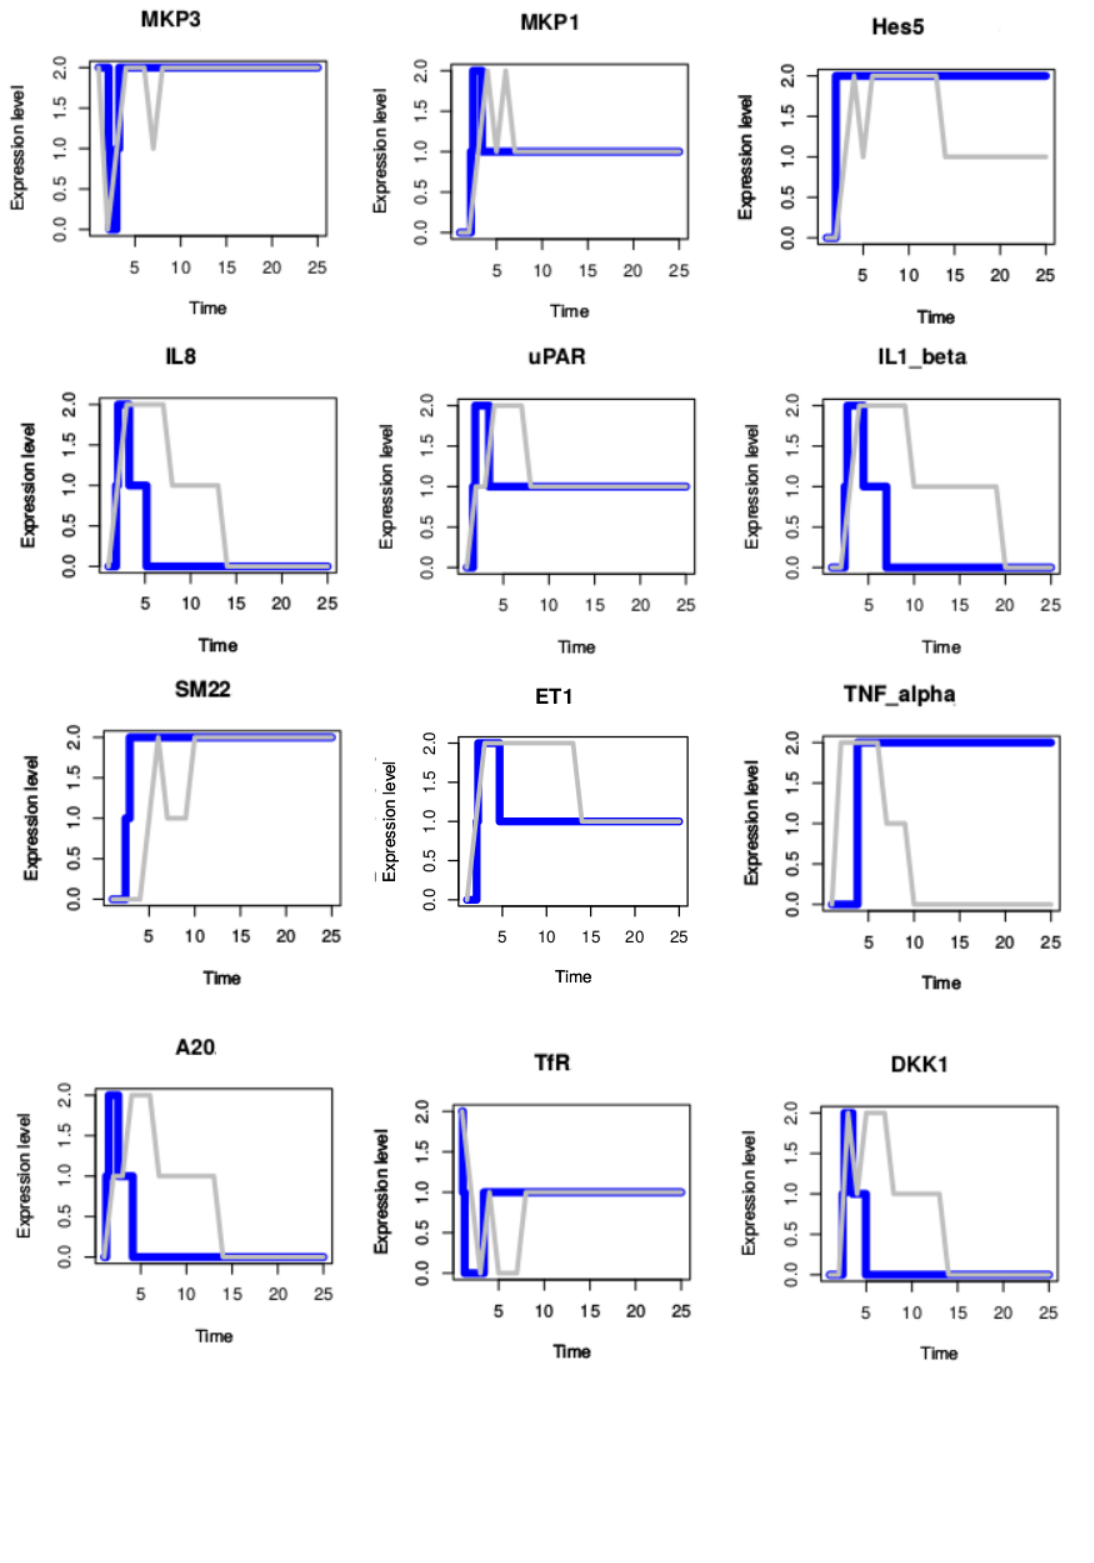
\includegraphics[width=5in,height=7in]{images/12genes_sim.png}
\caption{{\bf Results of simulations by introducing the synchronization sort.} The gray traces represent the experimental expected behaviors
from the discretization of the time-series data. The blue traces show the simulated behavior.}
\label{fig:rws}
\end{figure}


%%%%%images des noeuds clés

\subsubsection{Simulating biological processes.}
To validate our model, we studied the prediction of non-observed components of such a system and we focused on biological processes linked 
to Calcium stimulation, such as keratinocyte-differentiation, cell-adhesion and cell-cycle arrest.
Our results are shown in \pref{fig:knodes} and confirm literature experimental evidences on these processes.
In the case of keratinocyte-differentiation, this was a functional behavior measured on the cultured cells upon Calcium stimulation,
 so there was experimental evidences of this effect before measuring the gene expression.  
In the case of cell-cycle arrest, the switch-on of this component represents the fact that the E-cadherin stimulated model predicts the stop 
of growth, as confirmed by literature in human and mouse keratinocytes~\cite{Kolly2005}.
Finally, the cell-adhesion component is predicted to switch-on, also in according to published evidence~\cite{Tu2011} in human and mouse keratinocytes.

\begin{figure}[H]
\centering
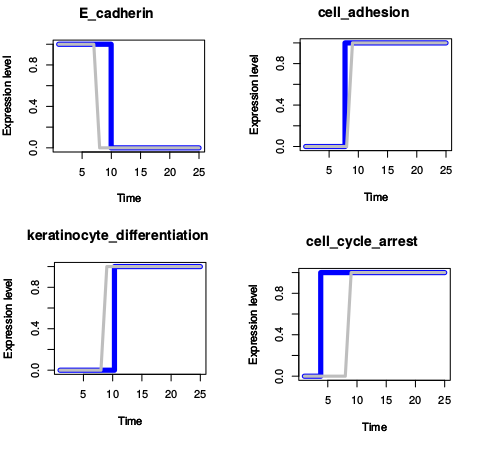
\includegraphics[width=4in,height=3.5in]{images/key_nodes1.png}
\caption{{\bf Results of the prediction of biological processes.} The gray traces represent the experimental and literature-based evidence.
The blue traces show the simulated behavior of E-cadherin and three biological processes.}
\label{fig:knodes}
\end{figure}

\subsection{Model validation: traces analysis}

To validate the results of the simulations, we automatically analyzed the traces generated by a set of $100$ simulations. Table \ref{traceAnalysis} shows the results
of the percentage of acceptance for the traces of each of the $12$ mRNA expressions. One can observe that there are $4$ components with a good 
acceptance rate ($> 76\%$), which are: A20, IL1$\_$beta, IL8, uPar;
$4$ traces with a good acceptance rate ($> 94\%$) when considering $1$ level of tolerance, which are: MKP1, MKP3, SM22, and TfR;
and finally $4$ traces, for which the model failed to predict their expressions:  ET1, Hes5, DKK1, and TNFa.
All in all, for this case study our model predicts relatively well, $8$ out of $12$, the experimental traces.
Errors on the prediction of the missing $4$ components may be because of missing regulatory interactions.

\begin{table}[!t]
\renewcommand{\arraystretch}{1.3}


\caption{Percentage of acceptance traces. First column represents the Automaton ($\mathcal{A}_{i}(w)$, where $\mathcal{A}_{i}$ is the Automaton and $w$ is the word recognized by $\mathcal{A}_{i}$) 
that is used to check if a given trace is accepted for a component in the second 
column. One can observe that many components can be recognized by the same Automaton. 
In the third column we show the percentage of accepted traces; in the fourth column, 
 the percentage of acceptance with a tolerance of one level ($T_{1}$).}


\label{traceAnalysis}
\centering
%table of result
\begin{tabular}{|c|c||c|c|}
\hline

\textbf{Automate}

&

\textbf{components}

&

\textbf{$\%$ of acceptance}

&

\textbf{$\%$ of acceptance $T_{1}$}
\\ \hline

$\mathcal{A}_{2}(01210)$

&

A20

&

91

&

100
\\ \hline

$\mathcal{A}_{2}(01210)$

&

IL1$\_$beta

&

81

&

100
\\ \hline

$\mathcal{A}_{2}(01210)$

&

IL8

&

93

&

100

\\ \hline

$\mathcal{A}_{2}(01210)$

&

TNF$\_$alpha

&

0

&

0

\\ \hline

$\mathcal{A}_{3}(01211)$

&

uPar

&

76

&

99

\\ \hline

$\mathcal{A}_{3}(01211)$

&

ET1

&

8

&

19

\\ \hline

$\mathcal{A}_{4}(0121210)$

&

DKK1

&

13

&

43

\\ \hline

$\mathcal{A}_{5}(0121211)$

&

Hes5


&

0

&

17

\\ \hline

$\mathcal{A}_{5}(0121211)$

&

MKP1


&

9

&

97

\\ \hline

$\mathcal{A}_{6}(0212)$

&

SM22


&

11

&

100

\\ \hline

$\mathcal{A}_{7}(02010)$

&

MKP3


&

11

&

98

\\ \hline

$\mathcal{A}_{8}(02121)$

&

Tfr


&

0

&

94

\\ \hline

 
\end{tabular}
\end{table}

\section{Conclusion}
This work describes the steps towards the integration of time-series data in large-scale cell-based models. 
We proposed an automatic method to build a timed and stochastic PH model from pathways of biochemical reactions present in 
the Pathway Interaction Database (PID). 
As a case-study we built a model combining signaling and transcription events relevant to keratinocyte differentiation induced by Calcium, which linked E-cadherin nodes and $12$ genes, which 
expression profiles was measured upon Calcium stimulation over time. The interaction graph represented by the model had $293$ nodes and $375$ edges.
We proposed a method to discretize time-series gene expression data, so they can be integrated to the PH simulations and logically explained by the PH stochastic analyses. 
Additionally, we implemented a method to automatically estimate the temporal and stochastic
parameters for the PH simulation, so this estimation process will not be biased by over fitting. 
Our results show that  we can observe dynamic effects on $11$ out of $12$ genes, for which $5$ of them represent accurate predictions, and $6$ of them missed few dynamic levels.
This error may be also a result from the incompleteness of the regulatory information in PID.
Moreover, when observing the predicted behavior of biological processes linked to Calcium stimulation, our predictions agreed with experimental and literature-based evidences.
Overall, with this work we show the feasibility of modeling and simulating large-scale networks with very few parameter estimation 
and having good quality predictions.
As perspectives of this work we intend to study the effects of computing automatically the concurrent rules on this system.
Also, we intend to improve the model prediction quality by empirically obtaining the dynamics of the system components by performing large stochastic simulations, as well 
as by implementing static analysis of quantitative properties by adding probabilistic features to the PH static solver.


\section{Acknowledgements}

This work was supported by a PhD grant from the CNRS and the French region \emph{Pays de la Loire} and grants from the German Ministry for Research and Education (BMBF) funding program MedSys (grant number FKZ0315401A) and AGENET (FKZ0315898).


%\bibliographystyle{plain}
%\bibliography{biblio.bib}
\begin{thebibliography}{10}

\bibitem{Ahmad08}
Jamil Ahmad, Olivier Roux, Gilles Bernot, Jean-Paul Comet, and Adrien Richard.
\newblock Analysing formal models of genetic regulatory networks with delays.
\newblock {\em International Journal of Bioinformatics Research and
  Applications (IJBRA)}, 4(3):240--262, 2008.

\bibitem{AMSW2012}
David~Spieler Aleksandr~Andreychenko, Linar~Mikeev and Verena Wolf.
\newblock Approximate maximum likelihood estimation for stochastic chemical
  kinetics.
\newblock {\em EURASIP Journal on Bioinformatics and Systems Biology}.

\bibitem{Batt15092010}
Gregory Batt, Michel Page, Irene Cantone, Gregor Goessler, Pedro Monteiro, and
  Hidde de~Jong.
\newblock Efficient parameter search for qualitative models of regulatory
  networks using symbolic model checking.
\newblock {\em Bioinformatics}, 26(18):i603--i610, 2010.

\bibitem{batt2007timed}
Gr{\'e}gory Batt, Ramzi~Ben Salah, and Oded Maler.
\newblock {\em On timed models of gene networks}.
\newblock Springer, 2007.

\bibitem{busch2008gene}
Hauke Busch, David Camacho-Trullio, Zbigniew Rogon, Kai Breuhahn, Peter Angel,
  Roland Eils, and Axel Szabowski.
\newblock Gene network dynamics controlling keratinocyte migration.
\newblock {\em Molecular systems biology}, 4(1):199, 2008.

\bibitem{chaouiya2003qualitative}
Claudine Chaouiya, Elisabeth Remy, Brigitte Moss{\'e}, and Denis Thieffry.
\newblock Qualitative analysis of regulatory graphs: a computational tool based
  on a discrete formal framework.
\newblock In {\em Positive Systems}, pages 119--126. Springer, 2003.

\bibitem{de2003genetic}
Hidde De~Jong, Johannes Geiselmann, C{\'e}line Hernandez, and Michel Page.
\newblock Genetic network analyzer: qualitative simulation of genetic
  regulatory networks.
\newblock {\em Bioinformatics}, 19(3):336--344, 2003.

\bibitem{gardner2003inferring}
Timothy~S Gardner, Diego Di~Bernardo, David Lorenz, and James~J Collins.
\newblock Inferring genetic networks and identifying compound mode of action
  via expression profiling.
\newblock {\em Science}, 301(5629):102--105, 2003.

\bibitem{guziolowski2012automatic}
Carito Guziolowski, Aristotelis Kittas, Florian Dittmann, and Niels Grabe.
\newblock Automatic generation of causal networks linking growth factor stimuli
  to functional cell state changes.
\newblock {\em FEBS Journal}, 279(18):3462--3474, 2012.

\bibitem{guziolowski2013exhaustively}
Carito Guziolowski, Santiago Videla, Federica Eduati, Sven Thiele, Thomas
  Cokelaer, Anne Siegel, and Julio Saez-Rodriguez.
\newblock Exhaustively characterizing feasible logic models of a signaling
  network using answer set programming.
\newblock {\em Bioinformatics}, 29(18):2320--2326, 2013.

\bibitem{heiner2008petri}
Monika Heiner, David Gilbert, and Robin Donaldson.
\newblock Petri nets for systems and synthetic biology.
\newblock In {\em Formal methods for computational systems biology}, pages
  215--264. Springer, 2008.

\bibitem{kauffman1969metabolic}
Stuart~A Kauffman.
\newblock Metabolic stability and epigenesis in randomly constructed genetic
  nets.
\newblock {\em Journal of theoretical biology}, 22(3):437--467, 1969.

\bibitem{Kolly2005}
C.~Kolly, M.~M. Suter, and E.~J. Muller.
\newblock {{P}roliferation, cell cycle exit, and onset of terminal
  differentiation in cultured keratinocytes: pre-programmed pathways in control
  of {C}-{M}yc and {N}otch1 prevail over extracellular calcium signals}.
\newblock {\em J. Invest. Dermatol.}, 124(5):1014--1025, May 2005.

\bibitem{macnamara2012state}
Aidan MacNamara, Camille Terfve, David Henriques, Beatriz~Pe{\~n}alver
  Bernab{\'e}, and Julio Saez-Rodriguez.
\newblock State--time spectrum of signal transduction logic models.
\newblock {\em Physical Biology}, 9(4):045003, 2012.

\bibitem{maurin2009modeling}
Myl{\`e}ne Maurin, Morgan Magnin, and Olivier Roux.
\newblock Modeling of genetic regulatory network in stochastic $\pi$-calculus.
\newblock In {\em Bioinformatics and Computational Biology}, pages 282--294.
  Springer, 2009.

\bibitem{mitsos2009identifying}
Alexander Mitsos, Ioannis~N Melas, Paraskeuas Siminelakis, Aikaterini~D
  Chairakaki, Julio Saez-Rodriguez, and Leonidas~G Alexopoulos.
\newblock Identifying drug effects via pathway alterations using an integer
  linear programming optimization formulation on phosphoproteomic data.
\newblock {\em PLoS computational biology}, 5(12):e1000591, 2009.

\bibitem{molloy1982performance}
Michael~K. Molloy.
\newblock Performance analysis using stochastic petri nets.
\newblock {\em Computers, IEEE Transactions on}, 100(9):913--917, 1982.

\bibitem{PMR10-TCSB}
{L}o{\"i}c {P}aulev{\'e}, {M}organ {M}agnin, and {O}livier {R}oux.
\newblock Refining dynamics of gene regulatory networks in a stochastic
  $\pi$-calculus framework.
\newblock In {\em Transactions on Computational Systems Biology XIII}, pages
  171--191. Springer, 2011.

\bibitem{Pinna2010}
Andrea Pinna, Nicola Soranzo, and Alberto de~la Fuente.
\newblock From knockouts to networks: Establishing direct cause-effect
  relationships through graph analysis.
\newblock {\em PLoS ONE}, 5(10):e12912, 10 2010.

\bibitem{porreca2010identification}
Riccardo Porreca, Eugenio Cinquemani, John Lygeros, and Giancarlo
  Ferrari-Trecate.
\newblock Identification of genetic network dynamics with unate structure.
\newblock {\em Bioinformatics}, 26(9):1239--1245, 2010.

\bibitem{priami1995stochastic}
Corrado Priami.
\newblock Stochastic $\pi$-calculus.
\newblock {\em The Computer Journal}, 38(7):578--589, 1995.

\bibitem{RAT2006}
R.~Altman S.~Reinker and J.~Timmer.
\newblock Parameter estimation in stochastic biochemical reactions.
\newblock {\em IEE Proceedings - Systems Biology}, 153, 2006.

\bibitem{schaefer2009pid}
Carl~F Schaefer, Kira Anthony, Shiva Krupa, Jeffrey Buchoff, Matthew Day, Timo
  Hannay, and Kenneth~H Buetow.
\newblock Pid: the pathway interaction database.
\newblock {\em Nucleic acids research}, 37(suppl 1):D674--D679, 2009.

\bibitem{Siebert06}
Heike Siebert and Alexander Bockmayr.
\newblock Incorporating time delays into the logical analysis of gene
  regulatory networks.
\newblock In {\em Computational Methods in Systems Biology}, volume 4210 of
  {\em LNCS}, pages 169--183. Springer, 2006.

\bibitem{snoussi1989qualitative}
El~Houssine Snoussi.
\newblock Qualitative dynamics of piecewise-linear differential equations: a
  discrete mapping approach.
\newblock {\em Dynamics and stability of Systems}, 4(3-4):565--583, 1989.

\bibitem{thieffry1995dynamical}
Denis Thieffry and Ren{\'e} Thomas.
\newblock Dynamical behaviour of biological regulatory networks—ii. immunity
  control in bacteriophage lambda.
\newblock {\em Bulletin of Mathematical Biology}, 57(2):277--297, 1995.

\bibitem{Thomas73}
Ren{\'e} Thomas.
\newblock Boolean formalization of genetic control circuits.
\newblock {\em Journal of Theoretical Biology}, 42(3):563 -- 585, 1973.

\bibitem{Tu2011}
C.~L. Tu, W.~Chang, and D.~D. Bikle.
\newblock {{T}he calcium-sensing receptor-dependent regulation of cell-cell
  adhesion and keratinocyte differentiation requires {R}ho and filamin {A}}.
\newblock {\em J. Invest. Dermatol.}, 131(5):1119--1128, May 2011.

\bibitem{van2013timed}
S~Van~Goethem, J-M Jacquet, Lubos Brim, and D~{\v{S}}afr{\'a}nek.
\newblock Timed modelling of gene networks with arbitrarily precise expression
  discretization.
\newblock {\em Electronic Notes in Theoretical Computer Science}, 293:67--81,
  2013.

\bibitem{yu2012hipathdb}
Namhee Yu, Jihae Seo, Kyoohyoung Rho, Yeongjun Jang, Jinah Park, Wan~Kyu Kim,
  and Sanghyuk Lee.
\newblock hipathdb: a human-integrated pathway database with facile
  visualization.
\newblock {\em Nucleic acids research}, 40(D1):D797--D802, 2012.

\end{thebibliography}



\appendix
 \section{Algorithm of patterns detection}

 Here are the algorithms that allow to detect and construct a process hitting model from an RSTC network.
 These algorithms have a polynomial time running that correspond to the running time of the procedure \ref{PatternDetection}.
 
 \begin{proposition}
  Algorithm \ref{PatternDetection} has a time complexity of $\mathcal{O}(|V|\log{}(h))$. 
  Where $h$ is the average height of the patterns in the RSTC network. In the worst case 
  $h = \log_{V}(|V|)$.
 \end{proposition}

 
 
 
 %%%%algorithm of patterns detection in all the network

%\begin{figure}[!t]
\begin{algorithm}
\begin{algorithmic}[1]
%\Procedure{patternDetection}{$Net,n$}\Comment{Given a node n, detect a set of minimal nodes that has a direct regulatory effect on n}
\REQUIRE $Net$ \COMMENT{The RSTC network}
\ENSURE generate the PH Model associated to $Net$
\FORALL{ Node $n$ in $Net$.getSetOfNodes() } 
\STATE $Pat$ = detectPattern ($Net$, $n$)
\STATE patternInPHModel ($out$, $Pat$)

\ENDFOR
%\STATE \textbf{return} $b$%\Comment{The gcd is b}
\end{algorithmic}
\caption{\bf: Algorithm for Pattern detection in an RSTC Network in order to generate the equivalent model in the PH formalism}
\label{automaticGenerationOfPHModel}
\end{algorithm}
%\end{figure}


%%%%%algorithm for detect the pattern of a given node

%\begin{figure}[!t]
\begin{algorithm}
\begin{algorithmic}[1]
%\Procedure{patternInPHModel}{$out,Pat$}\Comment{Write on the flux out the PH Model of a given pattern (Pat)}
\REQUIRE $Net$, $n$ \COMMENT{$Net$ is the network and $n$ is the current node}
\ENSURE Build a set of nodes associated to node $n$ that we call pattern.
%\WHILE{$r\not=0$}  %\Comment{We have the answer if r is 0}
\SWITCH {$n$}
 \CASE{TerminalNode} %\COMMENT{We compact many sub case of all terminal nodes}
   \STATE add node n to the pattern $Pat$
   \STATE numberPredecessor= $n$.getNumberOfPredecessor() %\COMMENT{To get the number of predecessor of node $n$}
   \SWITCH{numberPredecessor}
   
   \CASE{1}
    \FORALL {$p$ in setOfPredecessor (n)}
     \SWITCH {$p$}
    \CASE {TerminalNode}
      \STATE add node n to the pattern $Pat$
    \ENDCASE
    
    \CASE {TransientNode}
      \STATE detectPattern ($Net$, $p$);
    \ENDCASE
    
    \ENDSWITCH
   \ENDFOR
      \STATE Set the code of pattern $Pat$;
      \STATE return $Pat$;
   \ENDCASE
   
     \CASE {2}
     \STATE
     \ENDCASE
  % \DEFAULT
  %  \STATE \RETURN ERROR CODE \COMMENT{We can't treat this case}
  % \ENDDEFAULT
   \ENDSWITCH
\ENDCASE
   
   \CASE{TransientNode} %\COMMENT{We compact many sub case of all terminal nodes}
   %\STATE added node to the pattern
   \STATE numberPredecessor= $n$.getNumberOfPredecessor() %\COMMENT{To get the number of predecessor of node $n$}
   \SWITCH{numberPredecessor}
   
   \CASE{1}
    \FORALL {$p$ in setOfPredecessor (n)}
    \SWITCH {$p$}
    \CASE {TerminalNode}
      \STATE added node to the pattern $Pat$;
    \ENDCASE
    
    \CASE {TransientNode}
      \STATE detectPattern ($Net$, $p$);
    \ENDCASE
    
    \ENDSWITCH
   \ENDFOR
      \STATE Set the code of pattern $Pat$;
      \STATE return $Pat$;
   \ENDCASE
   
   \CASE {2}
   \STATE
   \ENDCASE
  % \DEFAULT
  %  \STATE \RETURN ERROR CODE \COMMENT{We can't treat this case}
  % \ENDDEFAULT
   \ENDSWITCH
 \ENDCASE
%\CASELINE {2}
%  \STATE Good-bye
%\DEFAULT
%  \STATE Again ?
%\ENDDEFAULT
\ENDSWITCH
%\ENDWHILE\label{euclidendwhile}
\end{algorithmic}
\caption{\bf: Algorithm for pattern detection, function detectPattern ($Net$, $n$)} \label{PatternDetection}
\end{algorithm}
%\end{figure}



%%%%%algorithm for write the pattern in PH model

%\begin{figure}[!t]
\begin{algorithm}
\begin{algorithmic}[H]

\REQUIRE $out$, $Pat$ \COMMENT{Pat is The pattern to be translated into the PH Model, out is the output file}
\ENSURE The correspondent PH Model of the given pattern Pat will write into the file $out$

\STATE $nocp$ = $Pat$.getNumberOfComponents() \COMMENT{Number of the components of the pattern $Pat$}
\STATE $tabPat$ = $Pat$.getTableOfPattern() \COMMENT{return the components of the pattern in $tabPat$}
\SWITCH {$nocp$}
 \CASE {2}
  \SWITCH {$code$}
 \CASE {A}
  \STATE out.write ($tabPat[1]$ 1 $\rightarrow$ $tabPat[0]$ $0$ $1$ $r_{a}$ $sa_{a}$);  \COMMENT{Component $tabPat[1]$ activates component $tabPat[0]$ with $r = r_{a}$ and $sa = sa_{a}$ }     
\ENDCASE
\CASELINE {I}
  \STATE out.write ($tabPat[1]$ 0 $\rightarrow$ $tabPat[0]$ $1$ $0$ $r_{i}$ $sa_{i}$);  \COMMENT{Component $tabPat[1]$ inhibits component $tabPat[0]$ with $r = r_{i}$ and $sa = sa_{i}$ }  

\ENDSWITCH
   
   
\ENDCASE

\CASE {3}
  \SWITCH {$code$}
 \CASE {C}
   \STATE out.write (coop ([$tabPat[2]$;$tabPat[1]$)] $\rightarrow$ $tabPat[0]$ $0$ $1$); \COMMENT{Cooperation between $tabPat[1]$ and $tabPat[2]$ to activate $tabPat[0]$}
        
\ENDCASE
\CASELINE {S}
  \STATE out.write (coop ([$tabPat[2]$;$tabPat[1]$)] $\rightarrow$ $tabPat[0]$ $0$ $1$); \COMMENT{Synchronization between $tabPat[1]$ and $tabPat[2]$ to activate $tabPat[0]$}
\DEFAULT
 \STATE out.write ((*unknow pattern*));
 \ENDDEFAULT
\ENDSWITCH
   
   
\ENDCASE

\ENDSWITCH

\end{algorithmic}
\caption{\bf: Algorithm for writing a given pattern into a file, function patternInPHModel ($out$, $Pat$)} \label{PHModelGeneration}
\end{algorithm}




%\begin{thebibliography}{4}

%\end{thebibliography}


\end{document}
